
%%% Local Variables: 
%%% mode: latex
%%% TeX-master: t
%%% End: 

\chapter{基于 $k$-CBP 碰撞检测算法}
\label{cha:kcbp-collision-detection}

碰撞检测算法是计算机图形学、计算机动画等领域里必不可少的基础算法之一。
本章提出了基于~$k$-CBP~的碰撞检测算法,算法首先对输入的网格模型进行预处理,构造模型的包围盒即~AABB~包围体、$k$-CBP,
当进行碰撞检测时,首先判断包围盒是否相交,若相交再进行~$k$-CBP~之间的相交测试,再次相交再进行实际模型的相交测试。
在进行实际模型的相交测试时,利用了~AABB~树形结构进行判断剪枝,
在~$k$-CBP~之间分别用~AABB~树的方式和基于~GJK~算法两种方式进行,实验结果表明本文提出的方法能够有效加速碰撞检测算法。

本章后续部分的内容组织如下:
第一节介绍了两种~$k$-CBP~之间的相交测试算法,分别是基于~AABB~树的方法和基于~GJK~的算法;
第二节介绍了三角网格之间的相交测试算法;
第三节介绍基于~$k$-CBP~的碰撞检测算法总体的流程;
然后是实验结果的分析以及小结。

\section{$k$-CBP~之间的相交测试算法}
\label{sec:kcbp:cd}

在所有基于包围体的碰撞检测算法中,都是利用了包围体的相交测试比直接用原始模型相交测试更简单以提升算法的整体效率,包围体的相交测试是非常重要的一个步骤。
与其他基于包围体的碰撞检测算法一样,本文基于~$k$-CBP~的算法也是先进行~$k$-CBP~的相交测试,若~$k$-CBP~相交,再进行原始模型的相交测试。
$k$-CBP~之间的相交测试以两种方法实现,一种是将构造的~$k$-CBP~进行空间划分,构造~$k$-CBP~的~AABB~树,再基于~AABB~树进行相交测试,详细划分原则等算法见第~\ref{subsec:kcbp:cd:aabb}~节;
另一种是基于计算凸多面体之间的最近距离的算法~GJK~,详细算法见第~\ref{subsec:kcbp:cd:gjk}节。

\subsection{基于 AABB 树的算法}
\label{subsec:kcbp:cd:aabb}

AABB~包围体是碰撞检测算法过程中一种最常用的包围体,构造模型的~AABB~包围体树能够有效提高模型的求交或碰撞检测过程。
本文将~$k$-CBP~视为普通的三角网格模型,采取一种自上而下的构造~AABB~包围体树的方法,顶层包围体为所有三角网格的包围体的并集,然后按照包围体跨度最大的维度进行划分成两个子节点,然后再对每个子节点进行递归划分,
具体算法如算法~\ref{alg:aabbtree:build}~所示。

\begin{algorithm}[htbp]
\small
\caption{AABB~树的构造}
\label{alg:aabbtree:build}
\begin{algorithmic}[1]
\Require
原始三角网格 $primitives$ 和下标 $first, last$
\Ensure
AABB~树的根节点 $root$

\Function{ConstructAABBTree}{$primitives, first, last$}
  \State $root \gets \Call{constructNode()}{}$ 
  \State $root.primitives \gets primitives$
  %\State $root.box \gets \emptyset $
  \For{$i = first \to last$}
      \State $root.box \gets root.box \cup primitives[i].box$
      \Comment{求每个三角网格的~AABB~的并集}
  \EndFor

  \State $size \gets primitives.size$  
  \If {$size = 1$}
  \State \Return $root$
  \EndIf

  \State $axis \gets \Call{longestAixs}{root.box}$
  \Comment {计算包围体跨度最大的轴}
  \State {$\Call{sort}{primitives, axis}$}
  \Comment {按照 $axis$ 对 $primitives$ 排序}
  
  \If {$size = 2 $}
      \State  {$root.left \gets \Call{constructNode()}{}$}
      \State  {$root.left.primitives \gets primitives[0]$}
      \State  {$root.left.box \gets primitives[0].box$}
      \State  {$root.right \gets \Call{constructNode()}{}$}
      \State  {$root.right.primitives \gets primitives[1]$}
      \State  {$root.right.box \gets primitives[1].box$}
      \State \Return $root$
  \EndIf
  \State $half \gets size / 2 $
  \State $root.left \gets \Call{ConstructAABBTree}{primitives, first, half}$
  \State \Comment{前一半作为其中一个叶子节点,继续递归构造}
  \State $root.right \gets \Call{ConstructAABBTree}{primitives, half+1, size}$ \Comment{后一半继续递归构造}
  \State \Return $root$
\EndFunction
\end{algorithmic}
\end{algorithm}

为了使生成的~AABB~包围体树更加平衡,因此划分策略为两个子节点包含相同数量的三角网格。划分轴采用沿着坐标轴方向节点跨度最大的轴进行划分,在对三角网格进行排序时,通常可选择三角网格中心位置的某轴向坐标值进行排序,
因为本文的策略为平衡二叉树策略,两个孩子节点包含三角网格数量一致,因此该点的选择不会对总体划分产生较大影响,只会影响划分轴边缘的三角网格,因此本文仅仅简单选择三角网格第一个坐标点的轴向坐标轴进行排序。

算法~\ref{alg:aabbtree:build}~的叶子节点为单个的三角网格,根据实际需要可以设置~AABB~树的最大深度,将达到最大深度的全部三角网格结合构成一个叶子节点。
假设算法~\ref{alg:aabbtree:build}~的时间复杂度为~$T(n)$~,则有
\begin{equation}
  T(n) = O(n \log n ) + 2T(\frac{n}{2}),
\label{equa:aabbtree:build}
\end{equation}
公式(\ref{equa:aabbtree:build})中~$O(n \log n)$~为算法中根据某坐标轴排序的耗费,根据主定理得此构造包围体树的整体算法时间复杂度~$T(n)=O(n\log^2n)$~,文献~\onlinecite{ericson2005real}~中提到可以用一种~$O(n)$~的算法替代其中的排序操作,使得整体复杂度为~$O(n\log n)$。

生成两个~$k$-CBP~的~AABB~包围体树后,当进行碰撞检测时,将采用算法~\ref{alg:aabbtree:traverse:iterator}~的迭代算法进行遍历判断。
从顶层~AABB~节点开始,若两个节点的~AABB~包围体相交,则进行深度优先遍历其孩子节点,当到达叶子节点时,再进行原生几何(本文中的~$k$-CBP~多边形网格,为了统一转化成与输入模型一致的三角网格)进行相交测试的判断,$k$-CBP~相交后,进行真实模型的相交测试也通过此方法进行。

\begin{algorithm}[htbp]
\small
\caption{基于AABB~树碰撞检测迭代算法}
\label{alg:aabbtree:traverse:iterator}
\begin{algorithmic}[1]
\Require
两棵~AABB~树的根节点 $rootA, rootB$
\Ensure
是否相交

\Function{TraverseDetection}{$rootA, rootB$}
  \State $p \gets \Call{initStack()}{}, q \gets \Call{initStack()}{}$  \Comment{初始化两个栈,用于记录待判断的~AABB~节点对}
  \State $p.\Call{Push}{rootA}, q.\Call{Push}{rootB}$  
  
  \While {$! p.\Call{empty()}{} ~~\textbf{and}~~ !q.\Call{empty()}{}$}
      \State $nodeA \gets p.\Call{Pop()}{}$
      \State $nodeB \gets q.\Call{Pop()}{}$
      \State $c \gets \Call{Intersect}{nodeA.box, nodeB.box}$ \Comment {判断两个节点的~AABB~包围体是否相交}
      \If {$c = \textbf{False}$}
          \State \textbf{Continue} \Comment{节点~AABB~不相交,则过滤到这两个节点及其孩子节点}
      \EndIf
      \If {$nodeA.\Call{isLeaf()}{}$}
          \If {$nodeB.\Call{isLeaf()}{}$}
              \Comment{两个叶子节点的原始几何进行相交测试} 
              \ForAll {$p_1 \in nodeA.primitives$}
                  \ForAll {$p_2 \in nodeB.primitives$}
                      \If {$\Call{Intersect}{p_1, p_2} = \textbf{True} $}
                          \State \Comment {按照第~\ref{sec:intersection:triangles}~节中的算法进行原始三角网格相交测试}
                          \State \Return \textbf{True} \Comment{若相交就直接返回True}
                      \EndIf
                  \EndFor
              \EndFor
          \Else  \Comment{nodeB~节点有孩子节点}
              \State $p.\Call{push}{nodeA}, q.\Call{push}{nodeB.left}$
              \State $p.\Call{push}{nodeA}, q.\Call{push}{nodeB.right}$
          \EndIf
      \Else \Comment{nodeA~节点有孩子节点}
          \If {$nodeB.\Call{isLeaf()}{}$}
              \Comment{nodeB~是叶子节点}
              \State $p.\Call{push}{nodeA.left}, q.\Call{push}{nodeB}$
              \State $p.\Call{push}{nodeA.right}, q.\Call{push}{nodeB}$
          \Else
              \Comment{nodeA~和~nodeB~都有叶子节点} 
              \State $p.\Call{push}{nodeA.left}, q.\Call{push}{nodeB.left}$
              \State $p.\Call{push}{nodeA.left}, q.\Call{push}{nodeB.right}$
              \State $p.\Call{push}{nodeA.right}, q.\Call{push}{nodeB.left}$
              \State $p.\Call{push}{nodeA.right}, q.\Call{push}{nodeB.right}$
          \EndIf
      \EndIf
  \EndWhile
  \State \Return \textbf{False} \Comment{遍历完毕也没有检测到原始三角网格相交,则返回False}
\EndFunction
\end{algorithmic}
\end{algorithm}

算法~\ref{alg:aabbtree:traverse:iterator}~中,底层叶子节点包含的原始三角网格数量与树的高度相关,对于相同的模型,树的高度越低,叶子节点包含三角网格数量也就越多,
且叶子节点测试的时间复杂度为~$O(m^2)$,$m$~为叶子节点包含的三角网格数量,一般而言在存储允许的情况下都尽量使得最底层叶子节点仅包含1个或少数几个三角形,以减少底层叶子节点三角网格两两测试的时间复杂度。

当在运动场景中的模型进行碰撞检测时,需要对~$k$-CBP及模型的~AABB~包围体树进行更新,本文采用一种近似的算法进行计算,详细将在第~\ref{sec:cd:baseon:kcbp}~节中介绍。

\subsection{基于 GJK 的算法}
\label{subsec:kcbp:cd:gjk}

GJK~算法是~E.G.Gilbert,D. W. Jonhson~和S.S. Keerthi(取三位作者姓名首字母作为算法名称的缩写)~等人在1988年发表的一种用于计算三维欧式空间中两个凸集合点之间的最近距离的方法\cite{gilbert1988fast},后常用于凸体之间的碰撞检测算法\cite{bergen1999fast}。本文也利用此算法用于计算两个凸包围多面体~$k$-CBP~之间的相交测试。

GJK~算法需要用到闵科夫斯基和(Minkowski Sum)如下定义:两个点集~$\mathbb{A}$~和~$\mathbb{B}$~,其~Minkowski~和为
%\begin{equation}
%  \mathbb{A} + \mathbb{B} = \{ \bm{a} + \bm{b} | \bm{a} \in \mathbb{A}, \bm{b} \in \mathbb{B}\},  
%  \label{}
%\end{equation}
~$\mathbb{A} + \mathbb{B} = \{ \bm{a} + \bm{b} | \bm{a} \in \mathbb{A}, \bm{b} \in \mathbb{B}\}$, 
将相应的加号改为减号得到~Minkowski~差,即~$\mathbb{A} - \mathbb{B} = \{ \bm{a} - \bm{b} | \bm{a} \in \mathbb{A}, \bm{b} \in \mathbb{B}\} $,GJK~算法的核心基础在于若两个凸体相交,则其~Minkowski~差必包含原点,因为若~$\mathbb{A}$~和
~$\mathbb{B}$~相交即~$\mathbb{A}$~和~$\mathbb{B}$~必含有公共交集,
即至少含有一点同时属于~$\mathbb{A}$~和~$\mathbb{B}$~,该点的~Minkowski~差即为原点~$(0, 0)$,
更加详细的原理和证明过程可以参考文献~\onlinecite{gilbert1988fast,bergen1999fast}。下面将以一个二维例子阐述此思想。

\begin{figure}[htbp]
\centering
\subcaptionbox{相交\label{fig:gjk:example:intersection}}{
  \includegraphics[width=.48\textwidth]{gjkIntersection.tikz}
} 
\subcaptionbox{不相交\label{fig:gjk:example:nonIntersection}}{
  \includegraphics[width=.48\textwidth]{gjkNonIntersection.tikz}
}
\caption{二维~GJK~算法示例}
\label{fig:gjk:example:2d}
\end{figure}

图~\ref{fig:gjk:example:intersection}~中,四个点坐标~$D(-4, 2), E(-2.5, 2), F(-2.5, 3.5), G(-4, 3.5)$~构成了四边形~$DEFG$~的四个顶点,
三角形~$ABC$~的坐标分别为~$A(-3, 1), B(-1,3), C(-3, 3)$~,
%其~Minkowski~差如式(\ref{equa:gjk:example:mink:diff})所示,
%\begin{equation}
%\label{equa:gjk:example:mink:diff}
%\Box_{DEFG} - \bigtriangleup_{ABC} = \left\{ 
%  \begin{array}{l}
%    (0.5, 1),  (-1.5, 0.5),  (0.5, 2.5), (-1, 2.5), \\ 
%    (-3, -1), (-1, -1),  (0.5, 0.5), (-1, 1), \\
%    (-3, 0.5), (0.5, -1), (-1.5, -1), (-1, 0.5)
%  \end{array}
%    \right\}  
%\end{equation}
其~Minkowski~差为~$\Box_{DEFG} - \bigtriangleup_{ABC} = \{  (0.5, 1),  (-1.5, 0.5),  (0.5, 2.5), (-1, 2.5),  (-3, -1),$\\$ (-1, -1),  (0.5, 0.5), (-1, 1),  (-3, 0.5),(0.5, -1), (-1.5, -1), (-1, 0.5) \}$,
四边形~$DEFG$~与三角形~$ABC$~相交,该~Minkowski~差构成的多边形~$H_1H_2H_3H_4H_5$~包含原点~$\bm{O}$。
而在图~\ref{fig:gjk:example:nonIntersection}~中,三角形坐标变为~$A'(-3, 1), B'(-1, 1), C'(-1,3)$,四边形~$DEFG$~坐标不变,
%其~Minkowski~差如式(\ref{equa:gjk:example:mink:diff2})所示,
%\begin{equation}
%\label{equa:gjk:example:mink:diff2}
%\Box_{DEFG} - \bigtriangleup_{A'B'C'} = \left\{ 
%  \begin{array}{l}
%   (0.5, 1), (-1.5, 1), (0.5, 2.5)  , (-1.5, -1), \\
%   (-1, 2.5),(-3, 2.5),  (-1.5, 2.5), (-3, 1),  \\
%   (-1.5, 0.5), (-3, 0.5), (-1, 1),(-3, -1) 
%  \end{array}
%  \right\}  
%\end{equation}
其~Minkowski~差为~$\Box_{DEFG} - \bigtriangleup_{A'B'C'} = \{  (0.5, 1), (-1.5, 1),  (0.5, 2.5)  , (-1.5, -1),  (-1, 2.5),$\\$(-3, 2.5),  (-1.5, 2.5), (-3, 1), (-1.5, 0.5), (-3, 0.5), (-1, 1),(-3, -1) \}$,
四边形~$DEFG$~与三角形~$A'B'C'$~不相交,该~Minkowski~差构成的多边形~$H_1'H_2'H_3'H_4'H_5'$不包含原点~$\bm{O}$。

通过该方法可将两个凸多边形或多面体是否相交转化为其~Minkowski~差是否包含原点,假设两个凸多边形或多面体分别有~$m$~和~$n$~个点,则直接计算其~Minkowski~差的时间复杂度为~$O(m \cdot n)$。
GJK~算法并不直接计算其~Minkowski~差,而是采取一种迭代的算法计算其~Minkowski~差一步一步向原点逼近,在有限步内若包含原点则原凸多边形或凸多面体相交反之不相交,文献~\onlinecite{bergen1999fast}~证明了该迭代过程能在有限步内完成。

GJK~算法中定义支持映射(Support Mapping)函数为将给定的方向~$\bm{d}$~映射为凸多边形或多面体中沿着~$\bm{d}$~方向最远的点,该点称为支持点(Support Point),用符号~$Support(\bm{d})$~表示,
该概念与本文第~\ref{sec:search:planes}节中搜索截面中的最大投影值点一致。设~$\mathbb{A}$~和~$\mathbb{B}$~的~Minkowski~差为~$\mathbb{D} = \mathbb{A}-\mathbb{B}$~,
则~$Support_\mathbb{D}(\bm{d}) = Support_\mathbb{A}(\bm{d}) - Support_\mathbb{B}(-\bm{d})$,这样能使得~Minkowski~差~$\mathbb{D}$~围成的区域更大并尽可能的包含原点。

GJK~算法采用如下的流程\cite{ericson2005real}进行迭代计算两个凸多面体~$\mathbb{A}$~和~$\mathbb{B}$~是否相交:

\begin{inparaenum}[(1)]
%\begin{enumerate}[(1)]
  \item 任选方向~$\bm{d}$~计算~$Support_\mathbb{D}(\bm{d}) = Support_\mathbb{A}(\bm{d}) - Support_\mathbb{B}(-\bm{d})$,即任意从~$\mathbb{A}$~和~$\mathbb{B}$~的~Minkowski~差中选择一点,加入集合~$\bm{S}$;\\ \indent
  \item 计算在~$ConvexHull(S)$~中,具有最小二范数的点即离原点最近的点~$\bm{D}$; \\ \indent
  \item 如果~$\bm{D}$~是原点本身或~$ConvexHull(S)$~包含原点,则表明$\mathbb{A}$~和~$\mathbb{B}$~相交,停止迭代;\\ \indent
  \item 规约集合~$\bm{S}$~,使得~$\bm{S}$~中是满足~$\bm{D}$~属于其凸包的最小的集合;\\ \indent
  \item 更新方向~$\bm{d} = -\bm{D}$~,并计算~$Support_\mathbb{D}(\bm{d}) = Support_\mathbb{A}(\bm{d}) - Support_\mathbb{B}(-\bm{d})$;\\ \indent
  \item 如果有新的$Support_\mathbb{D}(\bm{d})$~产生,则添加至集合~$\bm{S}$~并从第(2)步继续迭代,否则结束迭代,且得出~$\mathbb{A}$~和~$\mathbb{B}$~不相交的结论。
%\end{enumerate}
\end{inparaenum}

\begin{figure}[!ht]
\centering
\subcaptionbox{第一次迭代\label{fig:gjk:example:intersection:step1}}{
  \includegraphics[width=.48\textwidth]{gjkExampleIntersectionStep1.tikz}
} 
\subcaptionbox{第二次迭代\label{fig:gjk:example:intersection:step2}}{
  \includegraphics[width=.48\textwidth]{gjkExampleIntersectionStep2.tikz}
}
\subcaptionbox{第三次迭代\label{fig:gjk:example:intersection:step3}}{
  \includegraphics[width=.48\textwidth]{gjkExampleIntersectionStep3.tikz}
}
\caption{二维~GJK~算法迭代示例(相交情况)}
\label{fig:gjk:example:2d:intersection:iterator}
\end{figure}

具体而言,仍以图~\ref{fig:gjk:example:intersection}~为例,令四边形~$DEFG$~为~$\mathbb{A}$~,三角形~$ABC$~为~$\mathbb{B}$~,迭代过程如下:\\ \indent
\begin{inparaenum}[(1)]
\item 第一次迭代不妨设~$\bm{d_1} = (1,0)$,
如图~\ref{fig:gjk:example:intersection:step1}~所示,
%\begin{equation*}
%  \begin{array}{ll}
%    Support_\mathbb{D}(\bm{d_1}) & = Support_\mathbb{A}(\bm{d_1}) - Support_\mathbb{B}(-\bm{d_1}) \\
%                                 & = E(-2.5, 2) - A(-3,1)  = D_1(0.5, 1)
%  \end{array}
%  \label{euqa:gjk:step1}
%\end{equation*}
$Support_\mathbb{D}(\bm{d_1})  = Support_\mathbb{A}(\bm{d_1}) - Support_\mathbb{B}(-\bm{d_1})  = E(-2.5, 2) - A(-3,1) = D_1(0.5, 1),$
此时,$\bm{S} = \{D_1(0.5, 1)\}$;\\ \indent
\item 第二次迭代取~$\bm{d_2}=-\bm{D_1}=(-0.5, -1)$,如图~\ref{fig:gjk:example:intersection:step2}~所示,
%\begin{equation*}
%  \begin{array}{ll}
%  Support_\mathbb{D}(\bm{d_2})  & = Support_\mathbb{A}(\bm{d_2}) - Support_\mathbb{B}(-\bm{d_2}) \\
%                                & = D(-4, 2) - B(-1, 3)  = D_2(-3, -1)
%  \end{array}
%  \label{euqa:gjk:step2}
%\end{equation*}
$Support_\mathbb{D}(\bm{d_2})   = Support_\mathbb{A}(\bm{d_2}) - Support_\mathbb{B}(-\bm{d_2})  = D(-4, 2) - B(-1, 3) = D_2(-3, -1),$
此时,$\bm{S} = \{D_1(-0.5, 1), D_2(-3, -1)\}$;\\ \indent
\item 第三次迭代,计算~$ConvexHull(S)$~中最小二范数的点为~$I(-4/13, 7/13)$~,
并令~$\bm{d_3}=-\bm{I}=(4/13, -7/13)$,
%\begin{equation*}
%  \begin{array}{ll}
%  Support_\mathbb{D}(\bm{d_3})  & = Support_\mathbb{A}(\bm{d_3}) - Support_\mathbb{B}(-\bm{d_3}) \\
%                                & = E(-2.5, 2) - C(-3, 3)  = D_3(0.5, -1)
%  \end{array}
%  \label{euqa:gjk:step3}
%\end{equation*}
$ Support_\mathbb{D}(\bm{d_3})  = Support_\mathbb{A}(\bm{d_3}) - Support_\mathbb{B}(-\bm{d_3})  = E(-2.5, 2) - C(-3, 3) = D_3(0.5, -1),$
此时,$\bm{S} = \{D_1(0.5, 1), D_2(-3, -1), D_3(0.5, -1)\}$,
如图~\ref{fig:gjk:example:intersection:step3}~所示,$ConvexHull(S)$~为阴影部分覆盖区域,因其包含原点结束迭代,因此,$\mathbb{A}$~和~$\mathbb{B}$~相交。
\end{inparaenum}
%迭代过程如下:生成的公式高度高了,不好调整
%\begin{equation*}
%  \begin{array}{rl}
%    Support_\mathbb{D}(\bm{d_1}) & = Support_\mathbb{A}(\bm{d_1}) - Support_\mathbb{B}(-\bm{d_1}) \\
%                            & = E(-2.5, 2) - A(-3,1) = D_1(0.5, 1) \\
%    \bm{S} & = \{D_1(0.5, 1)\}, \bm{d_2}=-\bm{D_1}=(-0.5, -1) \\
%    Support_\mathbb{D}(\bm{d_2})  & = Support_\mathbb{A}(\bm{d_2}) - Support_\mathbb{B}(-\bm{d_2}) \\
%                            & = D(-4, 2) - B(-1, 3) = D_2(-3, -1) \\
%    \bm{S} &= \{D_1(-0.5, 1), D_2(-3, -1)\}, \bm{d_3}=-\bm{I}=(4/13, -7/13) \\
%    Support_\mathbb{D}(\bm{d_3})  & = Support_\mathbb{A}(\bm{d_3}) - Support_\mathbb{B}(-\bm{d_3}) \\
%                            & = E(-2.5, 2) - C(-3, 3)  = D_3(0.5, -1) \\
%    \bm{S} &= \{D_1(0.5, 1), D_2(-3, -1), D_3(0.5, -1)\}                 
%  \end{array}
%  \label{euqa:gjk:step1}
%\end{equation*}
%如图~\ref{fig:gjk:example:intersection:step3}~所示,$ConvexHull(S)$~为阴影部分覆盖区域,因其包含原点结束迭代,因此~$\mathbb{A}$~和~$\mathbb{B}$~相交。

\begin{figure}[htbp]
\centering
\subcaptionbox{第三次迭代\label{fig:gjk:example:nonIntersection:step3}}{
  \includegraphics[width=.48\textwidth]{gjkExampleNonIntersectionStep3.tikz}
} 
\subcaptionbox{第四次迭代\label{fig:gjk:example:nonIntersection:step4}}{
  \includegraphics[width=.48\textwidth]{gjkExampleNonIntersectionStep4.tikz}
}
\caption{二维~GJK~算法迭代示例(不相交情况)}
\label{fig:gjk:example:2d:intersection:iterator}
\end{figure}
再以图~\ref{fig:gjk:example:nonIntersection}~为例,设三角形$\mathbb{B'} = A'B'C'$,该例前两次迭代与上例相同,此处省略直接从第三次迭代起:\\ \indent
\begin{inparaenum}[(1)]
\item 第三次迭代,此时~$\bm{S} = \{(D_1', D_2') \}$,令~$\bm{d_3}=-\bm{I}=(4/13, -7/13)$,
%\begin{equation*}
%  \begin{array}{ll}
%  Support_\mathbb{D}(\bm{d_3})  & = Support_\mathbb{A}(\bm{d_3}) - Support_\mathbb{B'}(-\bm{d_3}) \\
%    & = E(-2.5, 2) - C'(-1, 3) = D_3'(-1.5, -1)
%  \end{array}
%  \label{euqa:gjk:non:step3}
%\end{equation*}
$ Support_\mathbb{D}(\bm{d_3})   = Support_\mathbb{A}(\bm{d_3}) - Support_\mathbb{B'}(-\bm{d_3}) = E(-2.5, 2) - C'(-1, 3)  = D_3'(-1.5, -1),$
此时$\bm{S} = \{D_1'(0.5, 1), D_2'(-3, -1), D_3(-1.5, -1)\}$,如图~\ref{fig:gjk:example:nonIntersection:step3}~所示,与上例不同,此时~$ConvexHull(S)$~并不包含原点,
所以规约集合~$\bm{S} = \{ (D_1'(0.5, 1), D_3'(-1.5, -1)\}$;\\ \indent
\item 第四次迭代,计算~$\bm{S}$~中二范数最小的点为~$I_2(-1/4, 1/4)$~,并令~$\bm{d}_4 = -I_2 = (1/4, -1/4)$,
%\begin{equation*}
%  \begin{array}{ll}
%  Support_\mathbb{D}(\bm{d_4})  & = Support_\mathbb{A}(\bm{d_4}) - Support_\mathbb{B'}(-\bm{d_4}) \\
%    & = E(-2.5, 2) - C'(-1, 3) \textrm{~或~} A'(-3, 1)  \\
%    & = D_3'(-1.5, -1) \textrm{~或~} D_1'(0.5, 1)
%  \end{array}
%  \label{euqa:gjk:non:step4}
%\end{equation*}
$Support_\mathbb{D}(\bm{d_4})   = Support_\mathbb{A}(\bm{d_4}) - Support_\mathbb{B'}(-\bm{d_4}) = E(-2.5, 2) - C'(-1, 3) \textrm{~或~} A'(-3, 1)   = D_3'(-1.5, -1) \textrm{~或~} D_1'(0.5, 1),$
此时,并没有新的~$Support_\mathbb{D}(\bm{d})$~产生,结束迭代,$\mathbb{A}$~和~$\mathbb{B}$~不相交。
\end{inparaenum}

在实际计算过程中,并不需要计算离原点最近即二范数最小的点的具体坐标值,只需选择垂直已有方向再进行判断选择方向即可,以图~\ref{fig:gjk:example:intersection:step3}~为例,
此时~$\overrightarrow{D_1D_2} = D_2(-3, -1) - D_1(0.5, 1) = (-3.5, -2)$,此时只需令~
$\bm{d_3'} = \overrightarrow{D_1D_2} \times \overrightarrow{D_1O} \times \overrightarrow{D_1D_2} = -(\overrightarrow{D_1D_2} \cdot \overrightarrow{D_1O})\overrightarrow{D_1D_2} +
(\overrightarrow{D_1D_2} \cdot \overrightarrow{D_1D_2})\overrightarrow{D_1O} = (5,-8.75)$
\footnote{$\bm{a} \times \bm{b} \times \bm{c} = -(\bm{c}\cdot\bm{b})\bm{a}+(\bm{c}\cdot\bm{a})\bm{b}$},
%\begin{equation*}
%  \begin{array}{ll}
%  Support_\mathbb{D}(\bm{d_3'})  & = Support_\mathbb{A}(\bm{d_3'}) - Support_\mathbb{B'}(-\bm{d_3'}) \\
%    & = E(-2.5, 2) - C(-3, 3) = D_3(0.5, -1) 
%  \end{array}
%\end{equation*}
$  Support_\mathbb{D}(\bm{d_3'})  = Support_\mathbb{A}(\bm{d_3'}) - Support_\mathbb{B'}(-\bm{d_3'})  = E(-2.5, 2) - C(-3, 3)  = D_3(0.5, -1),$
得到的~$Support_\mathbb{D}(d_3')$~仍为~$D_3(0.5,-1)$,与选择二范数最小点~$I$~所代表的方向达到相同的结果,因为选择二范数最小点的坐标代表方向与该垂直方向相同,因此结果一致。

判断原点是否被阴影部分面积所覆盖的过程如下:\\ \indent
%\begin{enumerate}[(1)]
\begin{inparaenum}[(1)]
  \item 通过$\bm{d}_3'$~得到的支持点$\bm{D}_3$中,$\bm{d}_3' \cdot \overrightarrow{OD_3} = (5, -8.75) \cdot (0.5, -1) = 11.25 > 0$~表明通过~$\bm{d}_3'$~方向到支持点的方向覆盖了原点,
    即原点在线段~$\overline{D_1D_2}$~线段的右下方;\\ \indent
  \item $\overrightarrow{D_3D_1}$~垂直并指向阴影部分面积方向为~$\overrightarrow{P_{D3D1}}=\overrightarrow{D_3D_1} \times \overrightarrow{D_3D_2} \times \overrightarrow{D_3D_1} = (-14, 0)$,此时,
    $\overrightarrow{P_{D3D1}} \cdot \overrightarrow{D_3O} = (-14, 0) \cdot (-0.5, 1) = 7 < 0$~表明原点~$\bm{O}$~在~$\overrightarrow{P_{D3D1}}$~的正方向即线段~$\overline{D_3D_1}$~的左边;\\ \indent
  \item 同时,$\overrightarrow{D_3D_2}$~垂直并指向阴影部分面积方向为~$\overrightarrow{P_{D3D2}}=\overrightarrow{D_3D_2}
\times \overrightarrow{D_3D_1} \times \overrightarrow{D_3D_2} = (0, 24.5)$
且~$\overrightarrow{P_{D3D1}} \cdot D_3O = (0, 24.5) \cdot (-0.5, 1) = 24.5 > 0$~表明原点~$\bm{O}$~在~$\overrightarrow{P_{D3D2}}$的正方向即线段~$\overline{D_3D_2}$~的上边;\\ \indent
%\end{enumerate}
\end{inparaenum}
以上三个条件全部满足,即原点~$\bm{O}$~被阴影部分所覆盖,即~$\mathbb{A}$~和~$\mathbb{B}$~的~Minkowski~差包含原点即可确定~$\mathbb{A}$~和~$\mathbb{B}$~相交,结束迭代。

相应的以图~\ref{fig:gjk:example:nonIntersection:step3}~为例,其结果仍保持一致。
%\begin{equation}
%  \begin{array}{ll}
%  Support_\mathbb{D}(\bm{d_3'})  & = Support_\mathbb{A}(\bm{d_3'}) - Support_\mathbb{B'}(-\bm{d_3'}) \\
%    & = E(-2.5, 2) - C'(-1, 3) \\
%    & = D_3'(-1.5, -1) 
%  \end{array}
%\end{equation}
$ Support_\mathbb{D}(\bm{d_3'})  = Support_\mathbb{A}(\bm{d_3'}) - Support_\mathbb{B'}(-\bm{d_3'}) = E(-2.5, 2) - C'(-1, 3) = D_3'(-1.5, -1)$,
图~\ref{fig:gjk:example:nonIntersection:step3}~中,
上一步通过~$\bm{d}_3'$~得到的支持点为~$D_3'(-1.5, -1)$,且$\overrightarrow{D_3'D_1'}$~垂直并指向阴影部分面积方向为~$\overrightarrow{P_{D_3'D_1'}}
\times \overrightarrow{D_3'D_2'} \times \overrightarrow{D_3'D_1'} =
(-2,-2)*(-3) + 8*(-1.5, 0) = (-6, 6)$,此时
~$\overrightarrow{P_{D3'D1'}} \cdot \overrightarrow{D_3'O} = (-6, 6) \cdot (1.5, 1) = -3 < 0$~表明下一次迭代方向需要以~$\overrightarrow{P_{D3'D1'}}$~的反方向开始,此时点~$D_2'$~可以规约掉,
即~$\bm{d}_4'= (6, -6)$,以此方向得到的支持点~$D_1'(0.5, 1)$,
此时,$\bm{d}_4' \cdot \overrightarrow{OD_1} = (6, -6) \cdot (0.5, 1) = -3 < 0 $ 表明通过~$\bm{d}_4'$~方向到支持点覆盖的区域没有包含原点,即可排除相交。

具体的算法如算法~\ref{alg:gjk}~所示,文献~\onlinecite{bergen1999fast}~证明了集合~$\bm{S}$~中在三维空间最多只包含4个点,且算法最终会收敛。
在实际实现过程中可以根据需求设定最大迭代次数,达到后或者认为没找到相交点或者采取保守态度进行下一步验证。

算法~\ref{alg:gjk}~第~12~行~$CHECKCONTAINUPDATE$~子过称需检测~$\bm{S}$~是否包含原点,必要时进行规约并获取下一次迭代方向,以上两个例子已经对二维情况进行分析,
具体三维实现可以参考文献~\onlinecite{bergen1999fast}。

\begin{algorithm}[!ht]
\small
\caption{基于~GJK~的~$k$-CBP~相交检测算法}
\label{alg:gjk}
\begin{algorithmic}[1]
\Require
两个$k$-CBP: $k\texttt{-}CBP_1, k\texttt{-}CBP_2$
\Ensure
是否相交
\Function{KCBPDetectionBasedOnGJK}{$k\texttt{-}CBP_1, k\texttt{-}CBP_2$}
    \State $\bm{d} \gets \Call{initNormal}$
    \State $\bm{D} \gets \Call{Support}{k\texttt{-}CBP_1, k\texttt{-}CBP_2, \bm{d}}$
    \State $S \gets \{p\}$
    \State $iter \gets 1 , \bm{d} \gets -\bm{d}$
    \While{$inter++ < MaxIter$}
        \State $\bm{D} \gets \Call{Support}{k\texttt{-}CBP_1, k\texttt{-}CBP_2, \bm{d}}$
        \If {$\bm{D} \cdot \bm{d} < 0 $}
            \State \Return \textbf{False}
        \EndIf
        \State $S \gets S \cup \bm{D}$
        \State $ contains \gets \Call{CheckContainUpdate}{S, \bm{d}}$ \Comment{检测是否包含原点,对集合~$S$~进行规约,并获取下一次迭代的方向~$\bm{d}$}
        \If {$contains$}
            \State \Return \textbf{True} \Comment{包含原点,直接返回相交,否则继续迭代}
        \EndIf
    \EndWhile
    \State \Return \textbf{False} \Comment{达到最大迭代次数,根据需求返回相交或者不相交}
\EndFunction
\end{algorithmic}
\end{algorithm}

\section{三角网格的相交测试算法}
\label{sec:intersection:triangles}

所有针对三角网格模型的碰撞检测算法最终都离不开三角网格的相交测试,不管模型是用何种包围体采用几何或者代数的方法都需要进行三角网格的相交测试。本文将利用一种几何代数相结合的方法进行三角网格之间的相交测试。
具体而言,假设两个不同面的三角形所在平面交于直线~$\bm{L}$~,两个三角形位置关系分为相交或者不相交两种情况,如图~\ref{fig:two:triangle:ui}所示。

\begin{figure}[!ht]
  \centering
    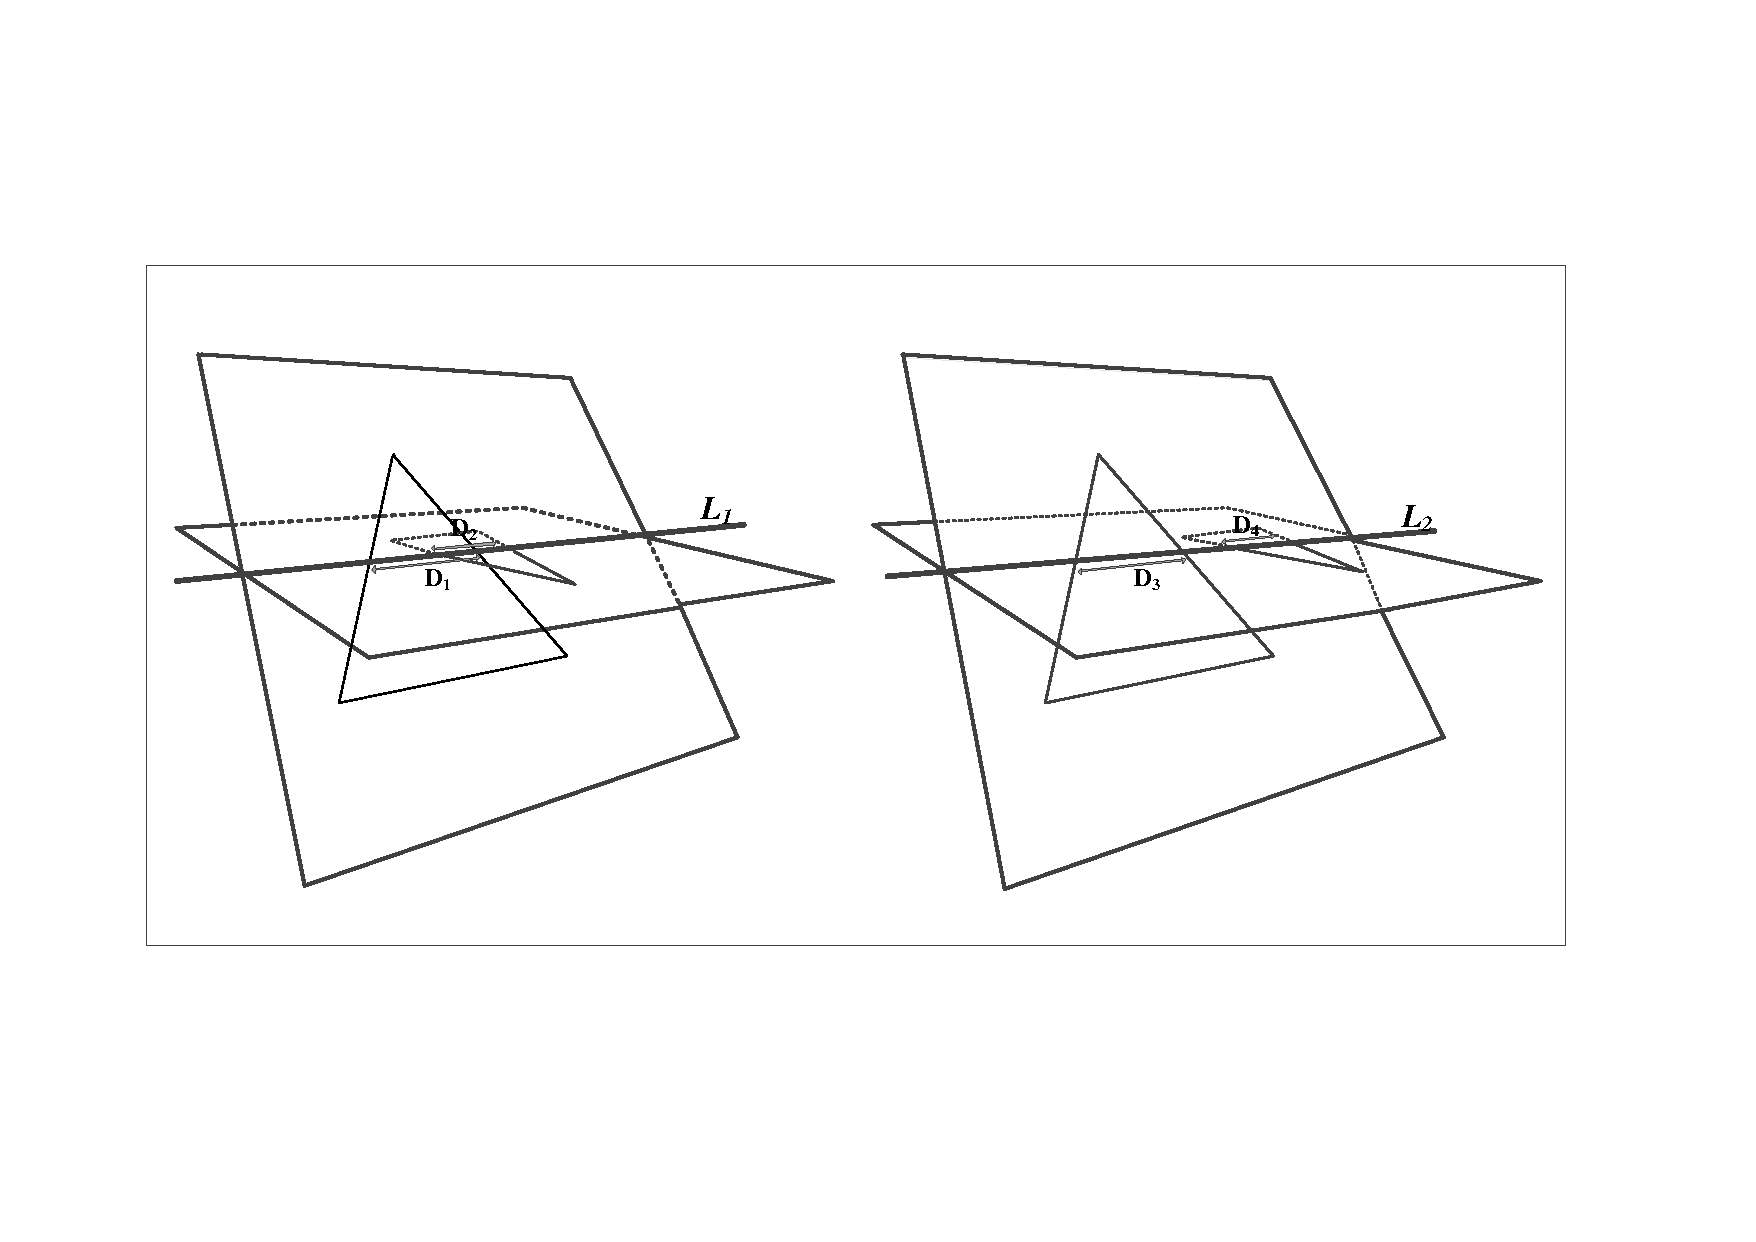
\includegraphics[width=4.5in]{TriangleTriangleTest.pdf}
    \caption{空间中两个非共面三角形的位置关系\cite{Moller1997}}
  \label{fig:two:triangle:ui}
\end{figure}

图~\ref{fig:two:triangle:ui}~左图中,两个三角形所在平面交于直线~$\bm{L}_1$~且与三角形公共部分为线段~$\bm{D}_1$~,另一个三角形与~$\bm{L}_1$~交于线段$\bm{D}_2$,相应的右图两个三角形分别交公共交线~$\bm{L}_2$~
于~$\bm{D}_3$~和~$\bm{D}_4$~,其中~$\bm{D}_1$~和~$\bm{D}_2$~相交可以推出两个三角形相交,反之因~$\bm{D}_3$~和~$\bm{D}_4$~不相交因此三角形不相交,因此只需要判断两个三角形与平面交线的线段是否相交即可\cite{Moller1997},
以下方法都基于此结论。

假设两个三角形~$T_1(\bm{U}_1,\bm{U}_2,\bm{U}_3), T_2(\bm{V}_1,\bm{V}_2,\bm{V}_3)$~所在平面分别为~$\Pi_1, \Pi_2$,相应的法向分别为~$\bm{n}_1, \bm{n}_2$,
假设平面方程~
\begin{equation}
  \Pi_1 = \bm{n}_1 \cdot \bm{x}+d_1 = (\bm{U_2} - \bm{U_1}) \times (\bm{U_3}-\bm{U_1})  \cdot \bm{x} + d_1,
\label{equa:tri:tri:plane}
\end{equation}
其中将任意一点~$U_i, i \in \{1,2,3\}$~带入公式(\ref{equa:tri:tri:plane})得~$d_1$,同理得到~$\Pi_2$。

然后将三角形~$T_2$~的三个顶点带入方程(\ref{equa:tri:tri:plane})得到~$T_2$~到~$\Pi_1$~的有向距离~$\bm{l}_{1i}, i \in \{1,2,3\}$,根据~$\bm{l}_{1i}$~的值分为下面三种情况讨论:\\ \indent
%\begin{enumerate}[(1)]
\begin{inparaenum}[(1)]
  \item 若~$\forall i \in \{1,2,3\}, l_{1i} = 0$,即三角形~$T_2$~的三个顶点到三角形~$T_1$~所在~$\Pi_1$~的距离都为$0$,则两个三角形共面;\\ \indent
  \item 若~$\forall i \in \{1,2,3\}, l_{1i} > 0$ 或~$\forall i \in \{1,2,3\}, l_{1i} < 0$,即三角形~$T_2$~的三个顶点到三角形~$T_1$~所在~$\Pi_1$~的有向距离同号,则~$T_2$~在~$\Pi_1$~的同一侧,可立即排除相交;\\ \indent
  \item 其他情况,三角形~$T_2$~必交~$\Pi_1$~于一条线段。
%\end{enumerate}
\end{inparaenum}

同理可以根据三角形~$T_1$~到三角形~$T_2$~所在平面~$\Pi_2$~得到类似的情况。针对情况(1),共面的两个三角形求交可以通过两个三角形中三条线段两两判定是否相交最多9次线段线段求交判定可得,或者通过我们在文献~\onlinecite{linjianli2014}~中提出的方法进行,该方法对线段三角形的位置做了详细的分类可通过不超过~6~次线段线段求交判定;针对情况(2),计算出有向距离同号后即可排除相交立即返回;
针对情况(3),如图~\ref{fig:two:triangle:ui2}~所示,不妨设在三角形~$T_1$~中,点~$\bm{V}_1, \bm{V}_2$~在平面~$\Pi_2$的一侧,$\bm{V}_3$~在另外一侧,
且点~$\bm{V}_1, \bm{V}_2$~在平面上投影点分别为~$\bm{K}_1,\bm{K}_2$,线段~$\bm{V}_1\bm{V}_2, \bm{V}_2\bm{V}_3$~与~$\bm{L}$~分别交于点~$\bm{I}_1,\bm{I}_2$,点~$\bm{V}_1,\bm{V}_2$~向直线~$\bm{L}$~的投影点分别为~$\bm{P}_1,\bm{P}_2$,
三角形~$T_1$~交于直线~$\bm{L}$~与线段~$\overline{I_1I_2}$。%,现在目的是求$I_1I_2$。

\begin{figure}[htbp]
  \centering
    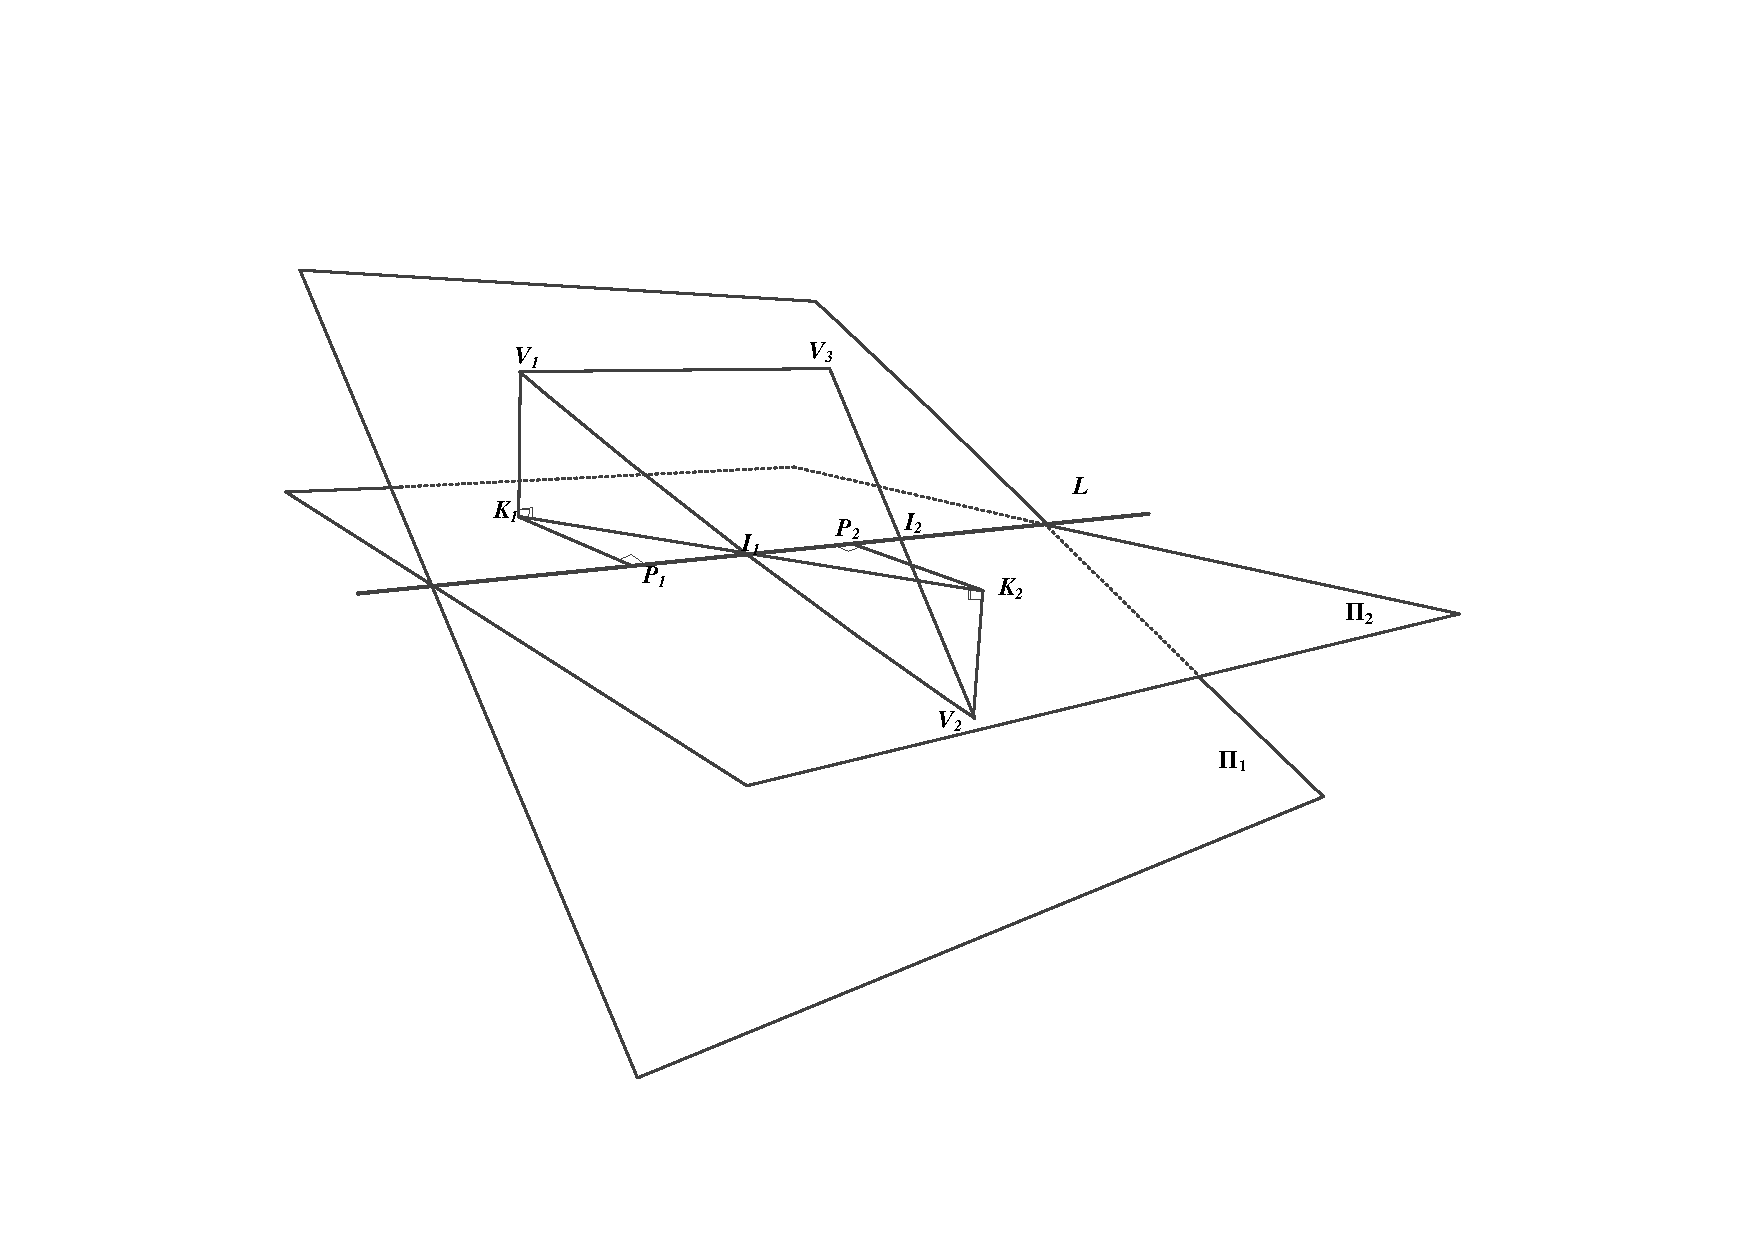
\includegraphics[width=3.5in]{TriangleTriangleTest2.pdf}
    \caption{求非共面三角形区间线段示意图\cite{Moller1997}}
  \label{fig:two:triangle:ui2}
\end{figure}

已知直线~$\bm{L}$~的方向为$\bm{n}_L = \bm{n}_1 \times \bm{n}_2$,设~$\bm{O}$~为~$\bm{L}$上一点,则直线的参数方程为
$\bm{L} = t \cdot \bm{n}_L + \bm{O}$~,假设交点~$I_1 = t_1 \cdot \bm{n}_L + \bm{O}$~,投影点满足
$p_1 = \bm{n}_L \cdot(\bm{V}_1 - \bm{O}), p_2 = \bm{n}_L \cdot (\bm{V}_2 - \bm{O})$,由图~\ref{fig:two:triangle:ui2}~可知,
$\bigtriangleup K_1P_1I_1 \sim \bigtriangleup K_2P_2I_1, \bigtriangleup V_1K_1I_1 \sim \bigtriangleup V_2K_2I_1$,可得
\begin{equation}
  \frac{t_1 - p_1}{p_2-p_1} = \frac{l_{11}}{l_{11}-l_{12}} \Rightarrow \newline
   t_1 = (p_2-p_1)\frac{l_{11}}{l_{11}-l_{12}} + p_1
  \label{equa:triangle:intersectionline:param}
\end{equation}

同理可得~$\bm{I}_2$~的参数~$t_2$,三角形~$T_2$~用相同的方法也能得到区间的参数,即可判断两个区间线段是否相交,进而可得该非共面的两个三角形是否相交。
完整的算法如~\ref{alg:triangles:intersection}~所示。

算法~\ref{alg:triangles:intersection}~第~10~行~在方法~$EDGEEDGETEST$~进行边边测试子过程中,可通过点与有向线段的位置关系确定,如线段两个端点都在另外一个有向线段的一边说明两线段不相交,反之则相交,不需要求解出具体的交点坐标。
在实际实现过程中,往往需要引入容差以提高算法的稳定性。文献~\onlinecite{Moller1997}~介绍了更多的优化技巧。

\begin{algorithm}[htbp]
\small
\caption{三角网格求交算法}
\label{alg:triangles:intersection}
\begin{algorithmic}[1]
\Require
两个三角形的6个顶点 $T_1(\bm{U}_1, \bm{U}_2, \bm{U}_3), T_2(\bm{V}_1, \bm{V}_2, \bm{V}_3)$
\Ensure
是否相交
\Function{TriangleTriangleDetection}{$\bm{U}_1, \bm{U}_2, \bm{U}_3, \bm{V}_1, \bm{V}_2, \bm{V}_3$}
    \State {$\Pi_1 \gets \bm{n}_1 \cdot \bm{x}+d_1$} \Comment{按照公式(\ref{equa:tri:tri:plane})计算$T_1$所在平面方程}
    \For {$i = 1 \to 3$}
        \State {$l_{1i} \gets \bm{n}_1 \cdot \bm{V}_i + d_1$} \Comment {计算$T_2$到$\Pi_1$的有向距离}
    \EndFor
    \If {$(l_{11} > 0 \textbf{~and~} l_{12} > 0 \textbf{~and~} l_{13} > 0) \textbf{or}
          (l_{11} < 0 \textbf{~and~} l_{12} < 0 \textbf{~and~} l_{13} < 0)$}
          \State \Return \textbf{False} \Comment{$T_2$在$\Pi_1$的同侧,排除}
    \EndIf
    \If {$l_{11} = 0 \textbf{~and~} l_{12} = 0 \textbf{~and~} l_{13} = 0$}
        \State \Return \Call{EdgeEdgeTest}{$\bm{U}_1, \bm{U}_2, \bm{U}_3, \bm{V}_1, \bm{V}_2, \bm{V}_3$}
        \State \Comment{$T_2$与$T_1$的共面,普通的边边相交测试}
    \EndIf
    \State {$\Pi_2 \gets \bm{n}_2 \cdot \bm{x}+d_2$} \Comment{按照公式(\ref{equa:tri:tri:plane})计算$T_2$所在平面方程}
    \For {$i = 1 \to 3$}
        \State {$l_{2i} \gets \bm{n}_2 \cdot \bm{U}_i + d_2$} \Comment {计算$T_1$到$\Pi_2$的有向距离}
    \EndFor
    \If {$(l_{21} > 0 \textbf{~and~} l_{22} > 0 \textbf{~and~} l_{23} > 0) \textbf{or}
          (l_{21} < 0 \textbf{~and~} l_{22} < 0 \textbf{~and~} l_{23} < 0)$}
          \State \Return \textbf{False} \Comment{$T_1$在$\Pi_2$的同侧,排除}
    \EndIf
    \State {$t_1 \gets \Call{CalParam}{}, t_2 \gets \Call{CalParam}$}  
    \Comment {按照公式(\ref{equa:triangle:intersectionline:param})计算线段$\bm{D}_1$的参数区间} 
    \State {$t_3 \gets \Call{CalParam}{}, t_4 \gets \Call{CalParam}$}  \Comment{类似的方法计算线段$\bm{D}_2$的参数区间} 
    \If {$\Call{Overlap}{t_1, t_2, t_3, t_4}$}
       \State \Return \textbf{True} \Comment{区间交叉,表明三角形相交返回\textbf{True}}
    \Else
       \State \Return \textbf{False}
    \EndIf
\EndFunction
\end{algorithmic}
\end{algorithm}

\section{基于 $k$-CBP 的碰撞检测算法}
\label{sec:cd:baseon:kcbp}

凸包围多面体可应用于加速相关算法的整体效率,图~\ref{lbl:bunny-box-kcbp-collsion-detection-example}
为利用~Bunny~模型进行碰撞检测的示例,图中编号为~1~与~2~的模型、2~与~3~的模型的包围盒分别相交, 而其~$16$-CBP~仅~1~与~2~相交,实际模型仅~1~与~2~相交。
用~$16$-CBP~可排除模型~2~与~3~之间的碰撞检测,而仅用包围盒算法则无法排除,显然检测模型~2~与~3~的~$16$-CBP~是否相交比直接通过检测模型~2~与~3~是否相交更省时间。
本文将从静止场景和运动场景两个角度来验证基于~$k$-CBP~的碰撞检测算法的有效性。 

\begin{figure}[htbp] 
\centering
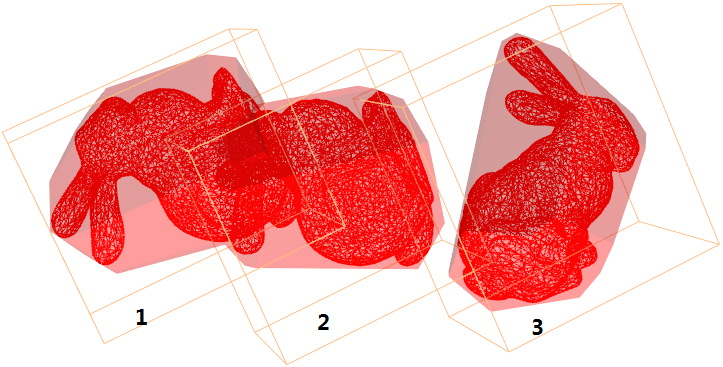
\includegraphics[width=4.5in]{bunny-box-kcbp-collsion-detection-example.png}
\caption{~$k-$CBP~应用于碰撞检测示例}
\label{lbl:bunny-box-kcbp-collsion-detection-example}
\end{figure}

\subsection{静止场景中的碰撞检测算法}
\label{subsec:static:cd}

模型的~$k$-CBP~相交后,会用模型的~AABB~树进一步对模型进行碰撞检测,模型的~AABB~树构造方法如第~\ref{subsec:kcbp:cd:aabb}~节所述,
图~\ref{fig:bunny:aabb:bvh:toplayer4}~是按照本文所采用的构造方法针对~Bunny~模型构造的~AABB~树形结构的顶上~4~层。

\begin{figure}[htpb]
  \centering
  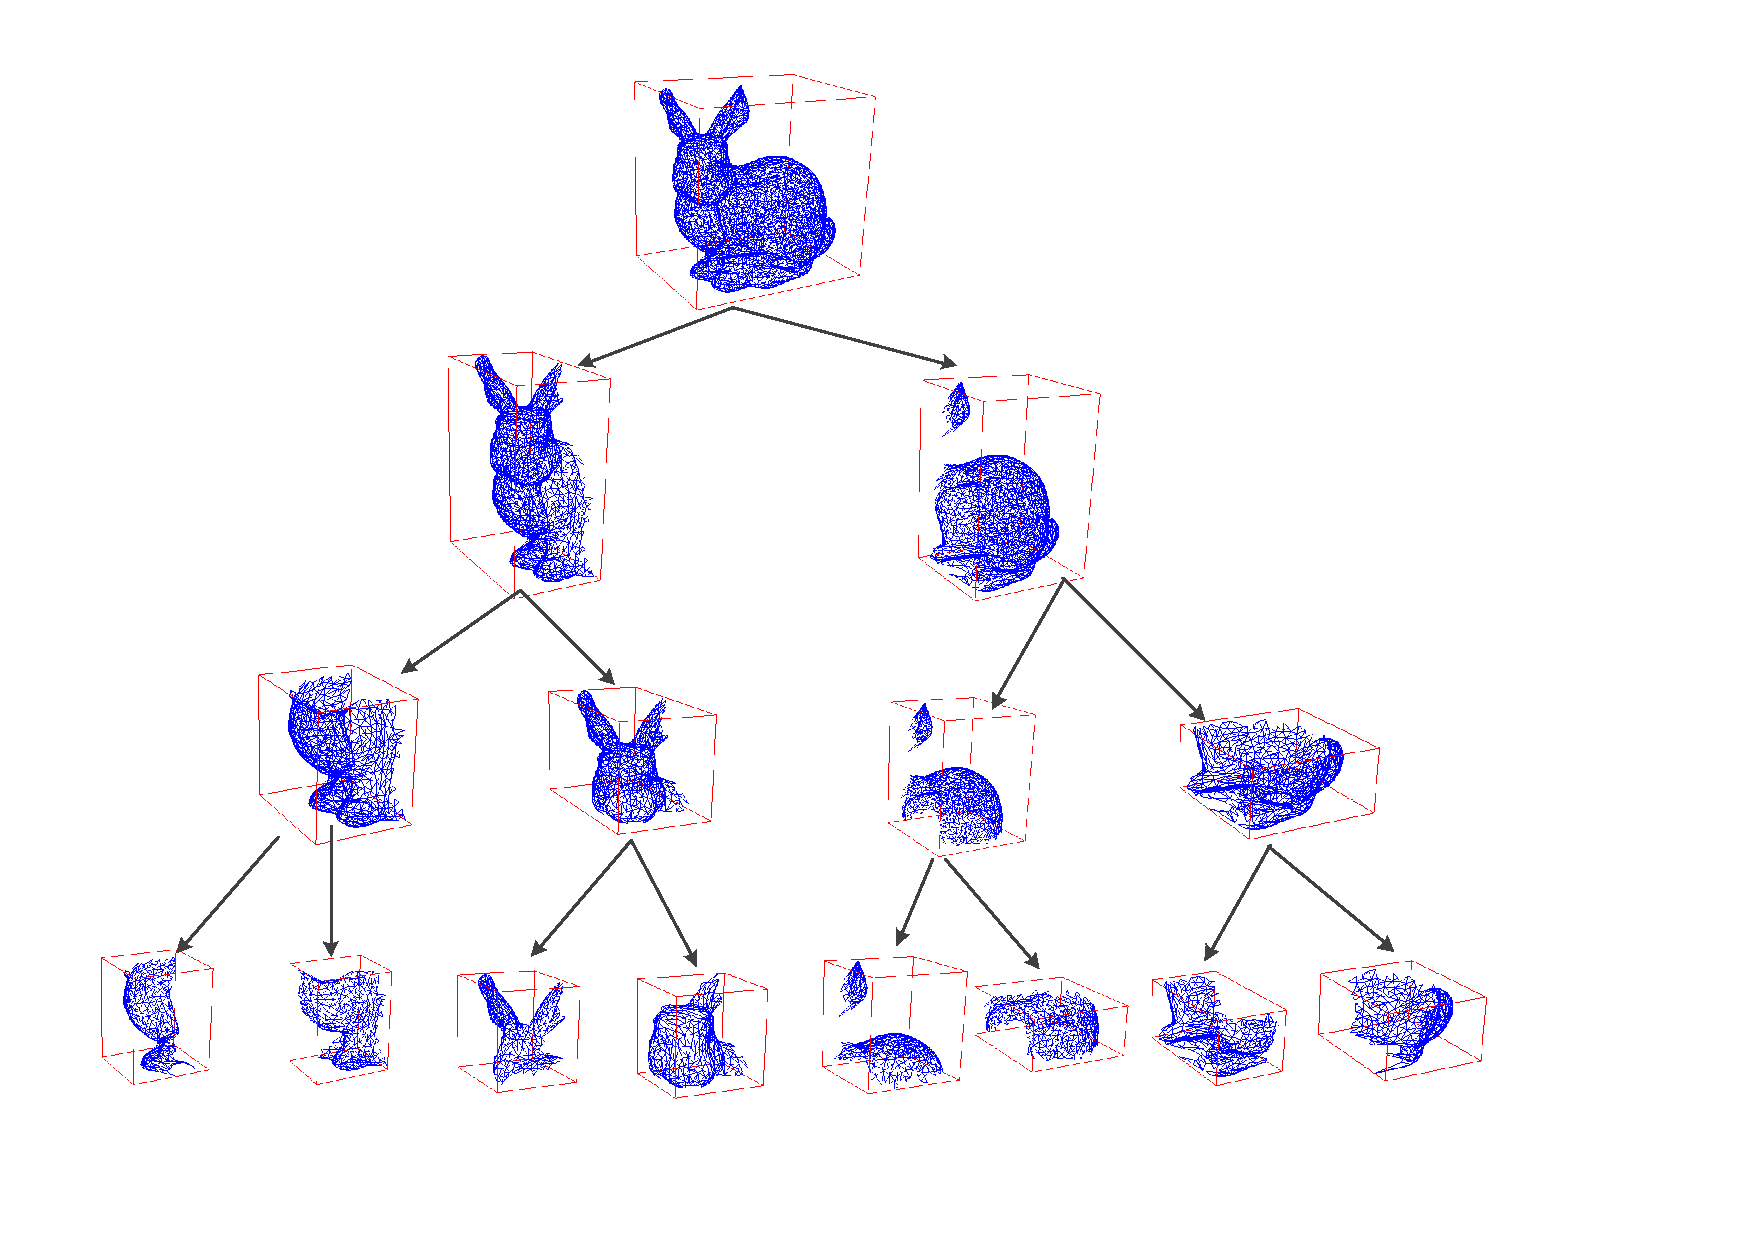
\includegraphics[width=\textwidth]{bunny-aabb-bvh-4-layers.pdf}
  \caption{Bunny~模型的~AABB~树形结构(部分)}
  \label{fig:bunny:aabb:bvh:toplayer4}
\end{figure}

\begin{figure}[htpb]
  \centering
  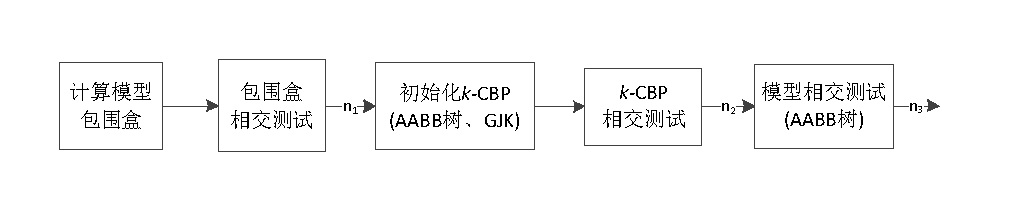
\includegraphics[width=\textwidth]{collision-detection-flowchart.pdf}
  \caption{基于~$k$-CBP~的碰撞检测算法流程图}
  \label{fig:flowchart:cd}
\end{figure}

整体的碰撞检测算法流程图如图~\ref{fig:flowchart:cd}~所示,首先扫描所有输入模型点集,对每个模型计算其包围盒,然后计算要参与碰撞检测的模型的包围盒对进行相交测试,
假设参与碰撞检测的模型的包围盒相交的对数为~$n_1$,再对这~$n_1$~对模型计算其~$k$-CBP~并进行初始化,如构造~$k$-CBP~的~AABB~树、初始化~GJK~算法,并计算~$k$-CBP~
是否相交,此步骤后剩余模型对数为~$n_2$,最后再对这~$n_2$~对模型进行构造~AABB~树进而进行相交测试,真实模型相交对数为~$n_3$。
整个流程中,包围盒的命中率为~$n_3 / n_1$,$k$-CBP~的命中率为~$n_3/n_2$。

\subsection{运动场景中的碰撞检测算法}
\label{subsec:moving:cd}

当在运动场景中的模型进行碰撞检测时,模型中的点坐标会更新,一种方法是重新计算模型中的所有点再以相同的流程和步骤对模型做碰撞检测,但当模型点数量较大时,耗时太久因此该方法不可取;
另外一种算法是仍然利用静止场景中的~AABB~树形结构,仅重新计算将要碰撞的节点的坐标值,进而进行相交检测。
节点包围盒坐标在运动过程中发生变化,精确的包围盒是重新计算该节点包含原始模型的点在变化后的点坐标值的包围盒,本文利用一种近似算法即仅对包围盒的~8~个顶点进行转换
然后计算这8个顶点的包围盒,用这个近似包围盒进行遍历剪枝,当到叶子节点后,再重新计算网格模型的点的新坐标值用同样的方法进行相交检测。

\begin{figure}[htbp]
  \centering
  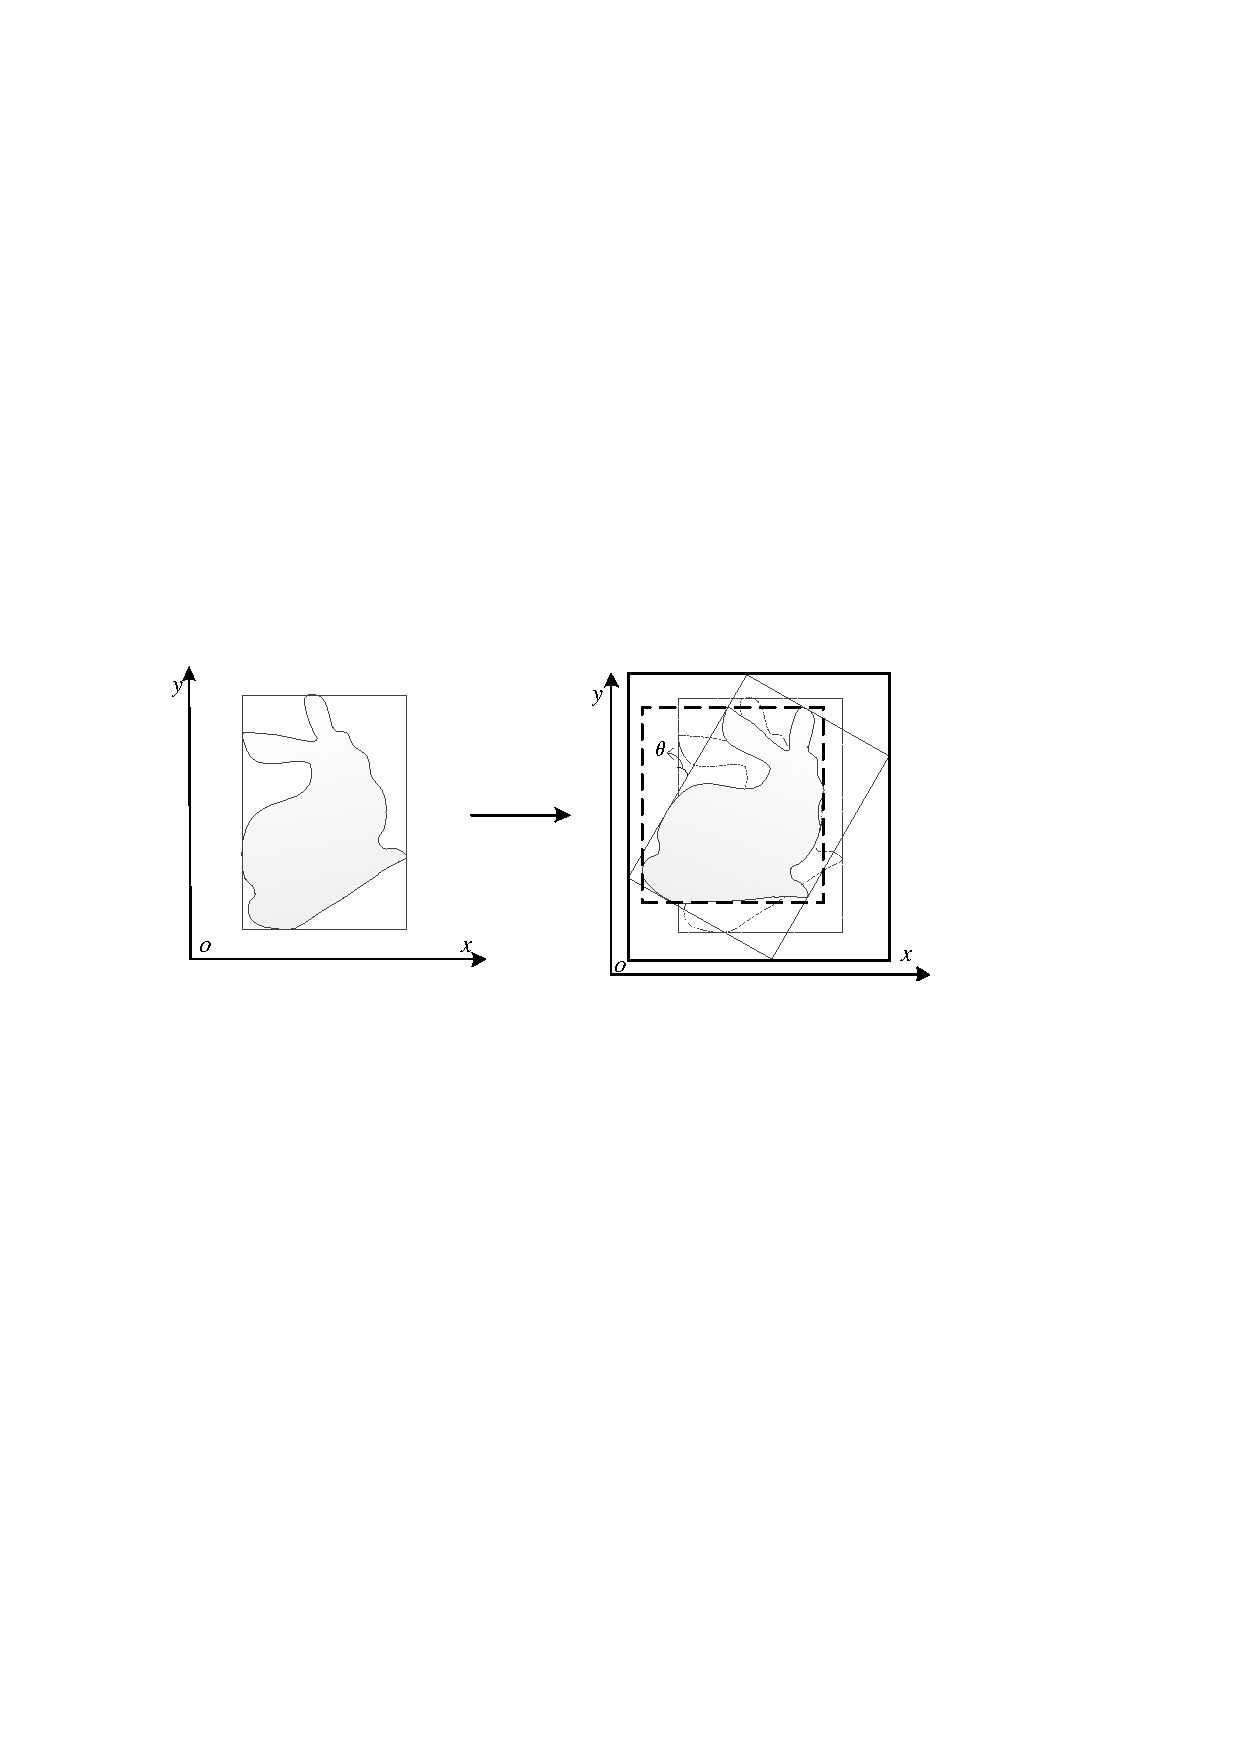
\includegraphics[width=.8\textwidth]{bunny-2d-AABB-Moving.pdf}
  \caption{AABB~更新策略示意图}
  \label{fig:bunny:moving}
\end{figure}

具体而言,以二维~Bunny~模型为例,如图~\ref{fig:bunny:moving}~所示,当模型顺时针旋转~$\theta$~后,本文利用近似算法得到新的包围盒如图中粗实线所示,而模型实际的包围盒为粗虚线所示,这样的结果会使得包围盒更不紧致,空白空间变得更大,
但速度更快,若包围盒相交后,会再用其~$k$-CBP~进行过滤,$k$-CBP~的顶点是精确顶点因而能更有效地进行过滤。

模型围绕任意过原点的轴~$\bm{n}(x, y,
z)$~旋转任意角度~$\theta$~的变换矩阵如式(\ref{equa:rotate:matrix})所示,其中$\lambda
= 1-\cos\theta$,
详细的推导过程可以参考文献~\onlinecite{dunn20023d}。
\begin{equation}
\left\{
    \begin{array}{ll}
    \bm{R}(\bm{n},\theta) 
    &= 
          \cos\theta \begin{pmatrix}
                      1 & 0 & 0 \\
                      0 & 1 & 0 \\
                      0 & 0 & 1
                     \end{pmatrix}
          + \lambda \begin{pmatrix}
                    \bm{n}_x^2 & \bm{n}_x\bm{n}_y & \bm{n}_x\bm{n}_z \\
                    \bm{n}_x\bm{n}_y & \bm{n}_y^2 & \bm{n}_y\bm{n}_z \\
                    \bm{n}_x\bm{n}_z & \bm{n}_y\bm{n}_z & \bm{n}_z^2 
                    \end{pmatrix}
          + \sin\theta \begin{pmatrix}
                      0 & \bm{n}_z & -\bm{n}_y \\
                      -\bm{n}_z & 0 & \bm{n}_x \\
                      \bm{n}_y & -\bm{n}_x & 0
                      \end{pmatrix}
          \\
    ~&=  
        \begin{pmatrix}
            %\begin{array}{ccc}
              %\cos\theta+(1-\cos\theta)\cdot\bm{n}_x^2 & (1-\cos\theta)\cdot\bm{n}_x\cdot\bm{n}_y + \sin\theta\cdot\bm{n}_z & (1-\cos\theta)\cdot\bm{n}_x\cdot\bm{n}_z-\sin\theta\cdot\bm{n}_y \\
              %(1-\cos\theta)\cdot\bm{n}_x\cdot\bm{n}_y-\sin\theta\cdot\bm{n}_z & \cos\theta+(1-\cos\theta)\cdot\bm{n}_y^2 & (1-\cos\theta)\cdot\bm{n}_y\cdot\bm{n}_z+\sin\theta\cdot\bm{n}_x \\
              %(1-\cos\theta)\cdot\bm{n}_x\cdot\bm{n}_z + \sin\theta\cdot\bm{n}_y & (1-\cos\theta)\cdot\bm{n}_y\cdot\bm{n}_z - \sin\theta\cdot\bm{n}_x &  \cos\theta+(1-\cos\theta)\cdot\bm{n}_z^2 
              \cos\theta+\bm{n}_x^2\lambda & \bm{n}_x\bm{n}_y\lambda + \bm{n}_z\sin\theta & \bm{n}_x\bm{n}_z\lambda-\bm{n}_y\sin\theta \\
              \bm{n}_x\bm{n}_y\lambda - \bm{n}_z\sin\theta & \cos\theta+\lambda\bm{n}_y^2 & \bm{n}_y\bm{n}_z\lambda+\bm{n}_x\sin\theta \\
              \bm{n}_x\bm{n}_z\lambda + \bm{n}_y\sin\theta & \bm{n}_y\bm{n}_z\lambda - \bm{n}_x\sin\theta &  \cos\theta+\bm{n}_z^2\lambda 
          \end{pmatrix} \\
  \end{array}
\right.
\label{equa:rotate:matrix}
\end{equation}

当模型平移时,点~$\bm{P}(x, y, z)$~平移~$\bm{t}(t_x, t_y, t_z)$~后的点坐标为~$\bm{P}'(x+t_x, y+t_y, z+t_z)$,可用~$4 \times 4$~的变换矩阵~$\bm{T}$~表示,即
\begin{equation}
  \bm{T}(\bm{t}) =
  \begin{pmatrix}
    1 & 0 & 0 & t_x \\
    0 & 1 & 0 & t_y \\
    0 & 0 & 1 & t_z \\
    0 & 0 & 0 & 1 \\
  \end{pmatrix}
  \label{equa:translate:matrix}
\end{equation}

因此当模型平移旋转时产生的变换矩阵~$\bm{M}$~为
\begin{equation}
\bm{M}=\bm{R}(\bm{n}, \theta) \cdot \bm{T}(\bm{t}),
\label{equa:transform:matrix}
\end{equation}

AABB~节点包围盒更新后的算法如算法~\ref{alg:transform:box}~所示,
算法输入为平移向量$\bm{t}$及旋转方向~$\bm{n}$~和角度~$\theta$~或者直接传入变化矩阵~$\bm{M}$~即可。

\begin{algorithm}[htbp]
\small
\caption{AABB节点包围盒更新算法}
\label{alg:transform:box}
\begin{algorithmic}[1]
\Require
AABB包围盒 $box$,
平移旋转变换矩阵$\bm{M}$
\Ensure
变换之后的包围盒 $box'$

\Function{TransformBox}{$box, \bm{M}$}
    \State $vertices \gets \Call{GetAABBVertices}{box}$ 
    \State $box' \gets \emptyset$
    \ForAll {$\bm{v} \in vertices$} \Comment{遍历~$box$~的8个顶点}
        \State {$\bm{v'}= \bm{M} \cdot \bm{v}$} \Comment{计算变换后的点坐标}
        \State $\Call{update}{box', \bm{v'}}$ \Comment{根据变换后的顶点~$\bm{v}$~更新$box'$}
    \EndFor
    \State \Return $box'$
\EndFunction
\end{algorithmic}
\end{algorithm}


\begin{algorithm}[!ht]
\small
\caption{运动场景中基于~AABB~树碰撞检测算法}
\label{alg:moving:cd}
\begin{algorithmic}[1]
\Require
两个模型~AABB~树的根节点 $root_0, root_1$ 及
平移旋转变换矩阵$\bm{M}$
\Ensure
模型是否相交 

\Function{MovingTraverseDetection}{$root_0, root_1, \bm{M}$}
    \State $mBox \gets \Call{TransformBox}{\bm{M}, root_0.box} $ \Comment{按照算法~\ref{alg:transform:box}~计算运动后的包围盒}
    \State $c \gets \Call{Intersect}{mBox, root_1.box} $
    \If {$c = \textbf{False}$}
        \State \Return \textbf{False} \Comment{包围盒不相交,直接返回\textbf{False}}
    \EndIf
    \If {$root_0.\Call{IsLeaf}$}
        \If {$root_1.\Call{IsLeaf}$} \Comment{两个叶子节点的原始几何进行相交测试} 
              \ForAll {$p_1 \in root_0.primitives$}
                  \ForAll {$p_2 \in root_1.primitives$}
                  \State \Return {$\Call{Intersect}{\bm{M}, p_1, p_2}$} \Comment{将$\bm{p}_1$应用于变换矩阵$\bm{M}$后采用算法\ref{sec:intersection:triangles}中进行三角网格相交测试}
                  \EndFor
              \EndFor 
        \Else
            \If {$\Call{MovingTraverseDetection}{root_0, root_1.left} \hspace{0.5em} \textbf{or} \newline \hspace{4em}
                \hspace*{5.5em} \Call{MovingTraverseDetection}{root_0, root_1.right}$} \hspace{2em}
                \State \Return \textbf{True}
            \EndIf
        \EndIf
    \Else
        \If {$root_1.\Call{IsLeaf}$}
            \If {$\Call{MovingTraverseDetection}{root_0.left, root_1} \hspace{0.5em} \textbf{or} \newline \hspace{4em}
                 \hspace*{5.5em} \Call{MovingTraverseDetection}{root_0.right, root_1}$}
            \State \Return \textbf{True}
            \EndIf
        \Else \Comment{两个节点都有孩子节点}
            \If {$\Call{MovingTraverseDetection}{root_0.left, root_1.left}  \hspace{0.5em} \textbf{or} \newline \hspace{4em}
                 \hspace*{5.5em} \Call{MovingTraverseDetection}{root_0.left, root_1.right} \hspace{0.5em} \textbf{or} \newline \hspace{4em}
                 \hspace*{5.5em} \Call{MovingTraverseDetection}{root_0.right, root_1.left} \hspace{0.5em} \textbf{or} \newline \hspace{4em}
                 \hspace*{5.5em} \Call{MovingTraverseDetection}{root_0.right, root_1.right}$}
                 \State \Return \textbf{True}
            \EndIf
      \EndIf
    \EndIf
    \State \Return \textbf{False}
\EndFunction
\end{algorithmic}
\end{algorithm}

运动场景中模型的碰撞检测算法如算法~\ref{alg:moving:cd}~所示,假设参与碰撞检测的两个模型中第一个运动且变换矩阵为~$\bm{M}$,第二个静止,
两个模型都运动时,可视第二个模型相对静止,将~$\bm{M}$~设置为第一个相对于第二个模型的相对变换矩阵。

算法~\ref{alg:moving:cd}~是一个递归算法,从~AABB~树的根节点起向底层叶子节点进行深度优先遍历,当检测到运动后的模型的某两个叶子节点的包围盒相交时,遍历其三角网格的相交检测算法,在实际实现过程中,本文的叶子节点仅含一个三角网格。
运动模型的三角网格应用变换矩阵得到一个新的三角网格,同样用~\ref{sec:intersection:triangles}~的算法对新的三角网格进行相交测试。
除了用该递归算法外,也可对算法~\ref{alg:aabbtree:traverse:iterator}~进行稍许改动(只需改变包围盒检测和三角网格检测的函数)的迭代算法,此处不在赘述。

在基于~GJK~的~$k$-CBP~碰撞检测算法中,只需要改变算法~\ref{alg:gjk}~中~$Support$~子过程,将变换矩阵应用到原始顶点进行计算得到新的支持点即可,而在连续运动的模型碰撞检测过程中,
利用爬山法可以将支持点的搜索优化到常数时间复杂度\cite{bergen1999fast}。


\section{实验结果}
\label{sec:exper-cd}
本章的实验主要分为3个部分,首先从~$k$-CBP~应用与碰撞检测的有效性上与仅用包围盒过滤算法进行对比,然后分别从静止场景和运动场景中与文献~\onlinecite{abenchmarking2007}中的基于~$k$-DOP~树的算法对比。
CollDet~\footnote{其源码和文档均可通过http://cgvr.cs.uni-bremen.de/research/colldet/~下载得到}是~Gabriel Zachmann~等人实现的一个碰撞检测库\cite{abenchmarking2007},内含基于~$k$-DOP~的实现,
在与~$k$-DOP~进行的实验对比结果中,本文在实验过程中均只通过~CPU~进行计算,针对碰撞检测实验环境中多个相同的实验模型\footnote{后文实验中用到的~HappyBuddha~模型和后文的~Hand~模型可从~http://cgvr.cs.uni-bremen.de/research/colldet\_benchmark/下载。},$k$-CBP~与~$k$-DOP~的构造均采用重新扫描扫描点集构造。

\subsection{与包围盒过滤算法对比}
\label{subsec:exper:box:kcbp}

本文实验通过生成不同数量的模型(模型位置和旋转角度随机生成),碰撞检测时首先判断包围盒是否相交, 然后判断凸包围多面体是否相交, 最后再判断实际模型是否相交。
该实验案例中模型和凸包围多面体是否相交都采用了普通~AABB~树的方式进行判断,
从如表~\ref{tab:exp:box:kcbp:collsiondetection}~的实验结果可看出含有凸包多围体的模型之间的碰撞检测算法能显著提高整体应用的效率. 

%\begin{landscape} 横放,效果不好看, 还是将表头的单位去掉了
\begin{table}[htbp]
\caption{$k$-CBP~和包围盒应用于碰撞检测结果对比}
\label{tab:exp:box:kcbp:collsiondetection}
\centering
\begin{tabular}{lccccccr}
 \toprule[1.5pt]
 \multirow{2}{*}{$n$} & CT(Box) & CT($16$-CBP) & DT(Box) & DT($16$-CBP) & r(Box) & r($k$-CBP) & \multirow{2}{*}{DP(Model)} \\
                      & (ms)    & (ms)          & (ms)  & (ms)          & (\%)      & (\%)  &   \\
  \midrule[1.0pt]
   10 & 0.1 & 1.8 &    26.0  & 0.1    & 0.00  & 100.00 & 0\\
   30 & 0.2 & 2.9 &   134.0  & 70.0   & 45.45 & 83.33 & 5\\
   50 & 0.5 & 4.8 &   506.0  & 255.2  & 46.34 & 86.36 & 19 \\
   70 & 0.4 & 4.8 &   901.1  & 492.5  & 44.16 & 80.95 & 34 \\
   90 & 0.7 & 5.7 &  1324.0  & 734.7  & 41.82 & 73.02 & 46 \\
  100 & 0.7 & 7.8 &  1481.0  & 870.7  & 43.31 & 75.34 & 55 \\
  150 & 1.0 & 9.8 &  4153.1  & 2473.0 & 42.98 & 70.75 & 150 \\
  200 & 1.6 & 12.8 & 8049.3  & 4430.9 & 41.02 & 71.32 & 281 \\
  \bottomrule[1.5pt]
 \end{tabular}
\end{table}
%\end{landscape}

如表~\ref{tab:exp:box:kcbp:collsiondetection}~所示,
其中~$n$~表示场景中模型的数量, CT(Box)、 CT($16$-CBP)~分别表示模型包围盒的构造时间(Construction Time,简称~CT)和凸包围16面体的构造时间\footnote{此处的时间为得到一个$k$-CBP后直接通过应用变换矩阵得到新的$k$-CBP总时间
且是利用~GPU~搜索截面的时间,后文与~$k$-DOP对比均采用~CPU~算法实现}, DT(Box)、DT($16$-CBP)~分表表示用包围盒进行碰撞检测和利用凸包围16面体进行碰撞检测所耗费的时间(Detection Time,简称~DT),
其中~r(Box)、r($16$-CBP)分别表示包围盒、16-CBP~的命中率(即用实际模型相交的数量除以包围体检测出来相交的数量), DP(Model)~检测到的模型实际相交的对数(Detection Pair,简称~DP),
显然计算模型包围盒所耗费的时间要明显少于计算凸包围多面体的时间,但由于凸包围多面体比包围盒紧致,
因而命中率比包围盒高,能排除更多本不相交的模型进而节省碰撞检测总时间,提高算法效率。该部分工作已经发表,详细内容见参考文献~\onlinecite{tanglei2014}。

\subsection{静止场景中与~$k$-DOP~算法对比}
\label{subsec:exper:kdop:kcbp:static}
在静止场景中的碰撞检测实验中,本文生成不同数量的模型,其位置和旋转角度随机生成($k$-DOP~和~$k$-CBP~采用相同的随机生成的数据),图~\ref{fig:static:cd:bunny}~为~Bunny~模型在模拟碰撞检测的实验实例。

\begin{figure}[htbp]
\centering
\subcaptionbox{n=10}{
  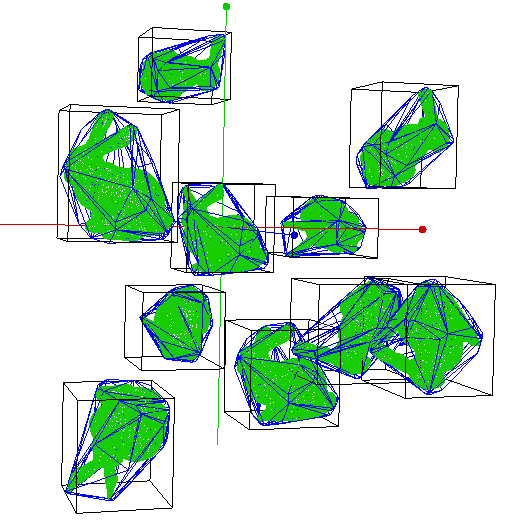
\includegraphics[width=.22\textwidth]{bunny-static-10.png}
} 
\subcaptionbox{n=20}{
  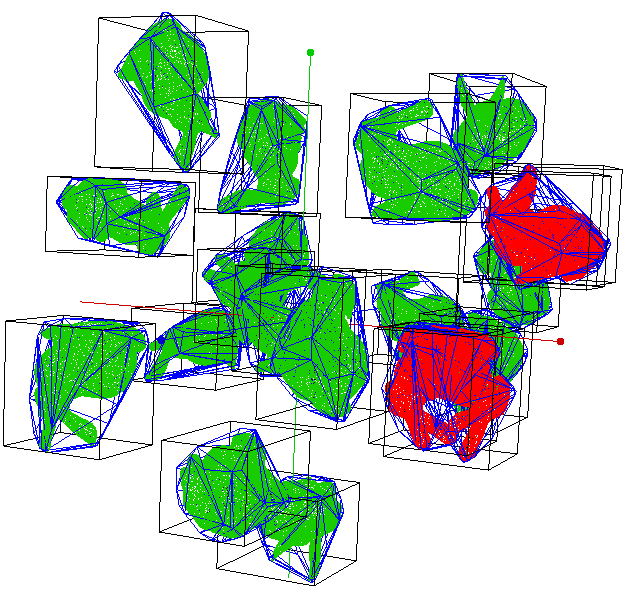
\includegraphics[width=.22\textwidth]{bunny-static-20.png}
}
\subcaptionbox{n=30}{
  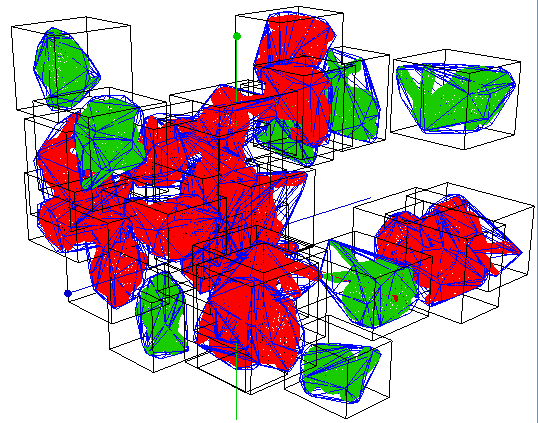
\includegraphics[width=.22\textwidth]{bunny-static-30.png}
}
\subcaptionbox{n=40}{
  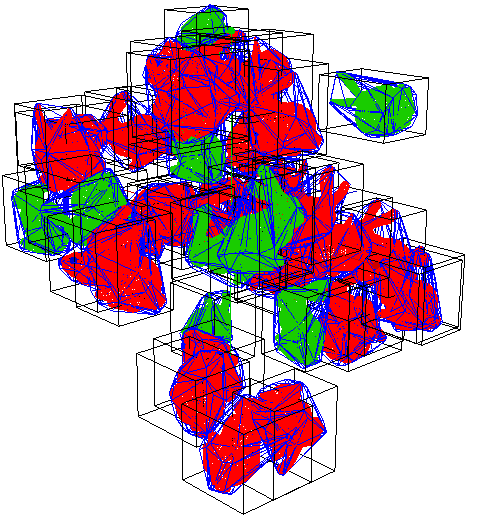
\includegraphics[width=.22\textwidth]{bunny-static-40.png}
}\\ 
\subcaptionbox{n=50}{
  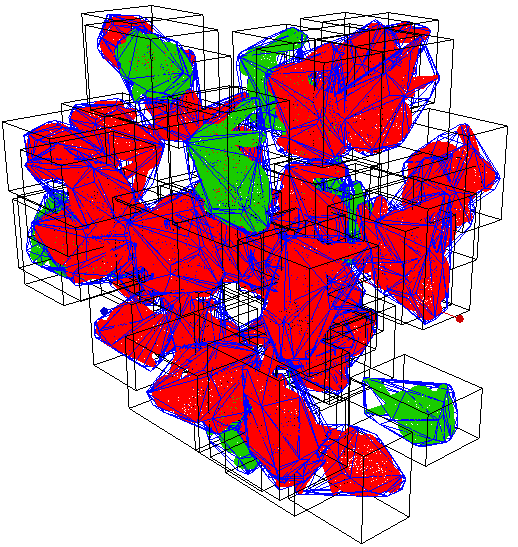
\includegraphics[width=.22\textwidth]{bunny-static-50.png}
}
\subcaptionbox{n=60}{
  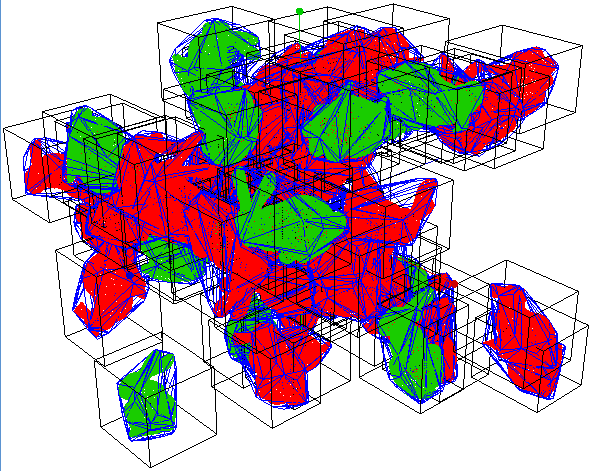
\includegraphics[width=.22\textwidth]{bunny-static-60.png}
}
\subcaptionbox{n=70}{
  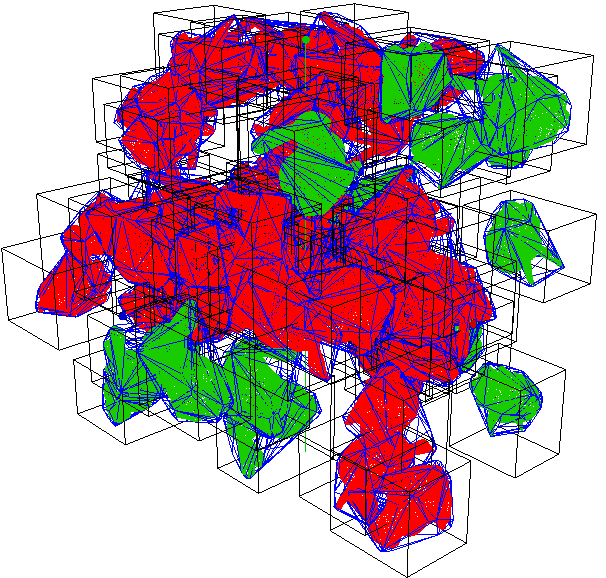
\includegraphics[width=.22\textwidth]{bunny-static-70.png}
}
\subcaptionbox{n=80}{
  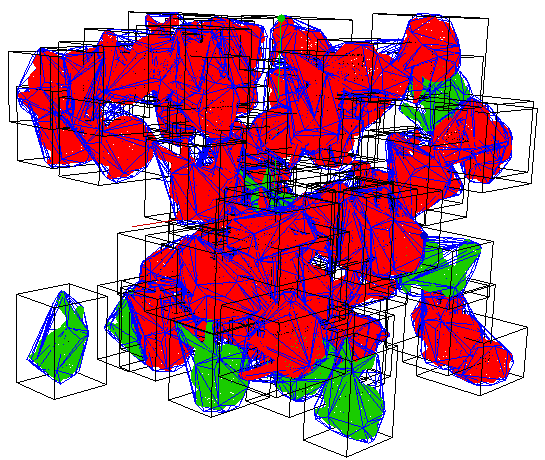
\includegraphics[width=.22\textwidth]{bunny-static-80.png}
}\\
\caption{静止场景下~Bunny~模型碰撞检测示例}
\label{fig:static:cd:bunny}
\end{figure}

表~\ref{tab:exp:bunny:k24:kdop:kcbp}~为本文算法与~$k$-DOP~均采用CollDet~中默认值~$k=24$~针对~Bunny~模型的实验结果。
其中,$n$~表示场景中模型的数量,$n$(Box)~表示通过包围盒过滤后构造碰撞检测对的有效模型数量,$n-n(\textnormal{Box})$~的值表示场景中模型的包围盒不与任何其他模型包围盒相交的模型数量,CT($k$-DOP)~和~CT($k$-CBP)~分别表示初始化的时间, CT($k$-DOP)~包括计算模型包围盒和计算$k$-DOP~树,CT($k$-CBP)~包括计算模型包围盒,
$k$-CBP~以及用于实际模型碰撞检测算法的~AABB~树,DT($k$-DOP)、DT($k$-CBP)($AABB$) 和~DT($k$-CBP)($GJK$)~均表示碰撞检测所耗费的时间, 
DT($k$-CBP)($AABB$)~为通过第~\ref{subsec:kcbp:cd:aabb}~节中介绍的~AABB~方法对~$k$-CBP~进行相交检测(包括构造~$k$-CBP~的~AABB~树所耗费的时间),
而~DT($k$-CBP)($GJK$)~表示通过第~\ref{subsec:kcbp:cd:gjk}~节中介绍的~GJK~方法对~$k$-CBP~进行相交检测,相应的时间都包括~$k$-CBP~相交后对模型进行~AABB~相交检测时间。

\begin{table}[!ht]  
\centering
\caption{静止场景下本文算法与~$k$-DOP~结果对比(Bunny)}
\label{tab:exp:bunny:k24:kdop:kcbp}
\begin{tabular}{cccccccc}
\toprule[1.5pt]
\multirow{2}{*}{$n$} & \multirow{2}{*}{$n$(Box)} & CT($k$-DOP) &  CT($k$-CBP) & DT($k$-DOP) & DT($k$-CBP) & DT($k$-CBP) \\%& \multirow{2}{*}{DP(Model)} \\ 
                     &                         &  (ms)        & (ms)         & (ms)        & $(AABB)$~(ms) & $(GJK)$~(ms)       \\
\midrule[1.0pt]
10 & 3 &	285.00 &	29.30      &0.01 &	0.01  & 	0.20  \\ %& 0  \\ 
20 & 10&	937.20 &	77.30      &0.60 &	0.70  & 	0.50  \\ %& 2  \\ 
30 & 24&	2233.60&	162.20     &2.00 &	2.00  & 	1.60  \\ %& 23 \\ 
40 & 38&	3522.20&	244.70     &1.80 &	2.10  & 	1.50  \\ %& 19 \\ 
50 & 46&	4238.20&	302.90     &2.60 &	3.10  & 	2.70  \\ %& 35 \\ 
60 & 59&	5447.60&	375.80     &4.00 &	5.00  & 	4.80  \\ %& 49 \\ 
70 & 68&	6271.00&	430.40     &5.20 &	5.20  & 	5.30  \\ %& 61 \\ 
80 & 78&	7186.20&	492.10     &6.60 &	6.90  & 	6.90  \\ %& 85 \\ 
90 & 88&	8096.20&	550.30     &8.20 &	8.70  & 	10.50 \\ %& 84 \\ 
100& 97&	8925.80&	615.00     &14.00&	10.60 & 	14.10 \\ %& 161\\ 
\bottomrule[1.5pt]
\end{tabular}
\end{table}

表~\ref{tab:exp:bunny:k24:kdop:kcbp:detail}~记录了更加详细的实验结果,其中~CT($k$-CBP)~和~CT(AABB)~分别表示本文算法中构造~$k$-CBP~的时间和构造用于具体模型碰撞检测算法的~AABB~树的时间,
DP(Box)~和~DP(Model)~表示包围盒相交的对数和实际模型碰撞的对数,这两组数据与~$k$-DOP~算法中相同,DP($k$-CBP)表示~$k$-CBP~相交的对数。
结合二表可知,在前期初始化碰撞检测环境中,本文算法优势明显,当模型为100时,$k$-DOP~算法构造~$k$-DOP~树需要近9秒的时间,而本文算法不到1秒,
初始化环境后,进入碰撞检测环节,本文算法较~$k$-DOP~相差不大,而本文提出的基于~AABB~树算法和基于~GJK~算法中,对于较少三角网格的~Bunny~模型而言,AABB~算法在静态环境中较~GJK~更优,
而从后文第~\ref{subsec:exper:kdop:kcbp:dynamic}~节也可以看出基于~GJK~算法在动态碰撞检测的环境中更优。 

\begin{table}[htbp]  
\centering
\caption{静止场景下本文算法实验结果(Bunny)}
\label{tab:exp:bunny:k24:kdop:kcbp:detail}
\begin{tabular}{cccccc}
\toprule[1.5pt]
$n$ & CT($k$-CBP)(ms) &  CT(AABB)(ms) & DP(Box) & DP($k$-CBP) & DP(Model)\\
\midrule[1.0pt]
10 &  13.60 &	16.60      & 2   &2   & 0  \\
20 &  23.80 &	53.40      & 10  &4   & 2  \\
30 &  35.00 &	128.00     & 42  &31  & 23 \\
40 &  42.40 &	199.40     & 42  &21  & 19 \\
50 &  51.00 &	244.20     & 66  &43  & 35 \\
60 &  58.00 &	313.40     & 121 &62  & 49 \\
70 &  66.80 &	360.20     & 144 &77  & 61 \\
80 &  72.20 &	412.80     & 167 &101 & 85 \\
90 &  81.00 &	463.80     & 261 &119 & 84 \\
100&  92.00 &	514.20     & 335 &200 & 161\\
\bottomrule[1.5pt]
\end{tabular}
\end{table}

\begin{figure}[!ht] 
\centering
\subcaptionbox{初始化时间对比\label{chart:exps:kdop:kcbp:bunny:init}}
{
    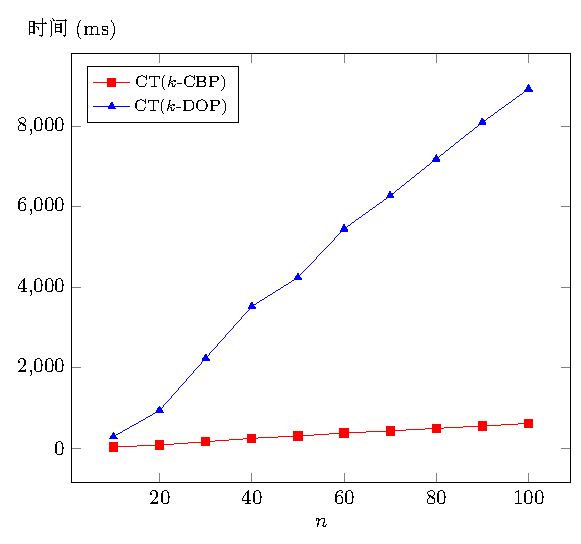
\includegraphics[width=0.45\textwidth,page=1]{staticcd.pdf}
}
\hspace{1em}
\subcaptionbox{碰撞检测时间对比\label{chart:exps:kdop:kcbp:bunny:cd}}
{  
   \includegraphics[width=0.43\textwidth,page=2]{staticcd.pdf}
}
\caption{静止场景下本文算法与~$k$-DOP~实验结果对比(Bunny)}
\label{chart:exps:kdop:kcbp:bunny}
\end{figure}

图~\ref{chart:exps:kdop:kcbp:bunny}~为本文的两种算法和文献~\onlinecite{abenchmarking2007,zachmann1998rapid}~中基于~$k$-DOP~的实现的实验结果的曲线展示图,
从图~\ref{chart:exps:kdop:kcbp:bunny:init}~可以看出,初始化构造~$k$-DOP~树和本文算法初始化所耗费时间与参与碰撞检测的模型的数量近线性关系,但明显本文算法所耗费时间更少,
图~\ref{chart:exps:kdop:kcbp:bunny:cd}~为初始化碰撞检测环境后进行碰撞检测所耗费的时间,本文的两种算法和基于~$k$-DOP~的算法相比,碰撞检测所耗费的时间相差不大,
总体来说针对~Bunny~模型而言,基于$k$-CBP~结合~AABB~树算法所耗费时间稍微较少,但三者相差不大,整体相差在~1--4~毫秒范围内。

\begin{figure}[htbp] 
\centering
\subcaptionbox{Bunny(4968个三角网格)\label{fig:exp:static:bunny}}
{  
   \includegraphics[width=\fourgraphicswidth\textwidth,page=3]{staticcd.pdf}
}
\subcaptionbox{Apple(8040个三角网格)\label{fig:exp:static:apple}}
{  
    \includegraphics[width=\fourgraphicswidth\textwidth, page=4]{staticcd.pdf}
}\linebreak %强制换行
\subcaptionbox{HappyBuddha(50000个三角网格)\label{fig:exp:static:happyBuddha}}
{  
   \includegraphics[width=\fourgraphicswidth\textwidth, page=14]{staticcd.pdf}
}
\subcaptionbox{Dinosaur(64546个三角网格)\label{fig:exp:static:dinosaur}}
{  
   \includegraphics[width=\fourgraphicswidth\textwidth, page=6]{staticcd.pdf}
}
\caption{静止场景下本文算法与~$k$-DOP~实验结果对比(k=24)}
\label{fig:chart:exps:kdop:kcbp:k24}
\end{figure}

图~\ref{fig:chart:exps:kdop:kcbp:k24}~记录了更多模型的实验结果,其中曲线三角形和正方形记录的是碰撞检测环境中的初始化时间,另外三条曲线分别是本文的两种算法和基于$k$-DOP~的算法碰撞检测所耗费的时间,左边纵坐标刻度为初始化时间,右边纵坐标刻度为碰撞检测的时间。
从中可得,在静态碰撞检测实验中,本文算法与基于$k$-DOP~的算法相比,在初始化环境过程中占用更少的时间,而在碰撞检测过程中针对不同的模型可能有不同的结果。从整体来看,本文算法优于基于~$k$-DOP~的算法。

\begin{figure}[htbp] 
\centering
\subcaptionbox{Bunny(4968个三角网格)\label{fig:exp:static:k46:bunny}}
{  
   \includegraphics[width=\fourgraphicswidth\textwidth,page=7]{staticcd.pdf}
}
\subcaptionbox{Apple(8040个三角网格)\label{fig:exp:static:k46:apple}}
{  
    \includegraphics[width=\fourgraphicswidth\textwidth, page=8]{staticcd.pdf}
}\linebreak %强制换行
\subcaptionbox{HappyBuddha(50000个三角网格)\label{fig:exp:static:k46:happyBuddha}}
{  
   \includegraphics[width=\fourgraphicswidth\textwidth, page=15]{staticcd.pdf}
}
\subcaptionbox{Dinosaur(64546个三角网格)\label{fig:exp:static:k46:dinosaur}}
{  
   \includegraphics[width=\fourgraphicswidth\textwidth, page=10]{staticcd.pdf}
}
\caption{静止场景下本文算法与~$k$-DOP~实验结果对比(k=46)}
\label{fig:chart:exps:kdop:kcbp:k46}
\end{figure}

对于更大的~$k$~值,构造层次结构的$k$-DOP~树时会耗费更多的时间和存储空间,在模型较大且模型数量较多时,以文献~\onlinecite{abenchmarking2007,zachmann1998rapid}~中最大的~$k$值为46~为例,例如当对~70~个~Dinosaur~模型进行构造~$k$-DOP~树时,32位应用程序已经会报内存不足的异常,且构造时间也更久,图~\ref{fig:chart:exps:kdop:kcbp:k46}~为~$k$-DOP~实现中的最大值~$k=46$~的实验结果。

更大的~$k$~值不一定能够使碰撞检测的效率提高,这与具体的碰撞检测环境有关,以~Bunny~模型和~Apple~模型为例,如图~\ref{fig:chart:exp:kdop:kcbp:k24:k46}~为~$k=24$~和~$k=46$~的结果对比,
其中,虚线的结果为~$k=46$~的结果,实现为~$k=24$~的结果,看出三种算法在~$k=24$~时碰撞检测所耗费的时间更少。因此在实际应用环境中应该根据具体的碰撞检测环境
选择不同的~$k$~值。

\begin{figure}[!ht] 
\centering
\subcaptionbox{Bunny(4968个三角网格)\label{fig:exp:static:k24:k46:bunny}}
{  
   \includegraphics[width=\fourgraphicswidth\textwidth,page=12]{staticcd.pdf}
}
\subcaptionbox{Apple(8040个三角网格)\label{fig:exp:static:k24:k46:apple}}
{  
    \includegraphics[width=\fourgraphicswidth\textwidth, page=13]{staticcd.pdf}
}
\caption{静止场景下不同~$k$~值实验结果对比}
\label{fig:chart:exp:kdop:kcbp:k24:k46}
\end{figure}

\subsection{运动场景中与~$k$-DOP~算法对比}
\label{subsec:exper:kdop:kcbp:dynamic}

对于运动场景中的碰撞检测实验,本文采取随机读入单个模型,并随机生成多个平移旋转变换构造多个模型,
然后令其中一个模型产生随机平移旋转变换进行运动,检测该运动模型与其他所有的模型进行碰撞检测,图~\ref{fig:dynamic:cd:bunny}~为随机产生的10个模型,
并让其中一个随机运动~7~步的示意图,示例中,对于没有和运动模型产生碰撞的模型,图中仅显示了其包围盒和~$k$-CBP。

\begin{figure}[!ht]
\centering
\subcaptionbox{$move=0$}{
  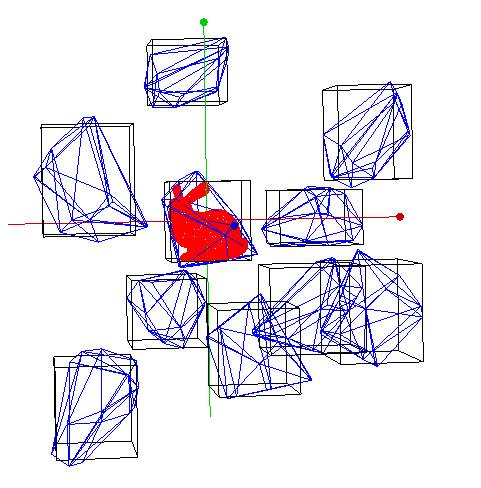
\includegraphics[width=.22\textwidth]{dynamic-bunny-m10-s0.png}
} 
\subcaptionbox{$move=1$}{
  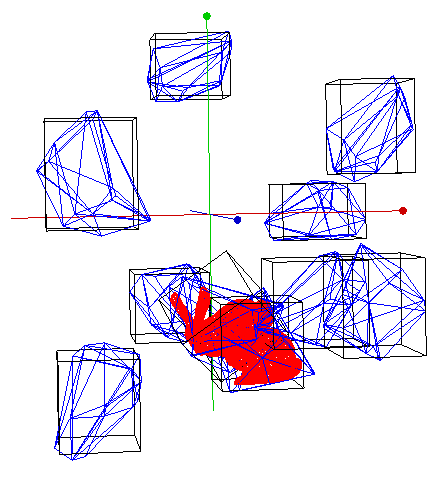
\includegraphics[width=.22\textwidth]{dynamic-bunny-m10-s1.png}
}
\subcaptionbox{$move=2$}{
  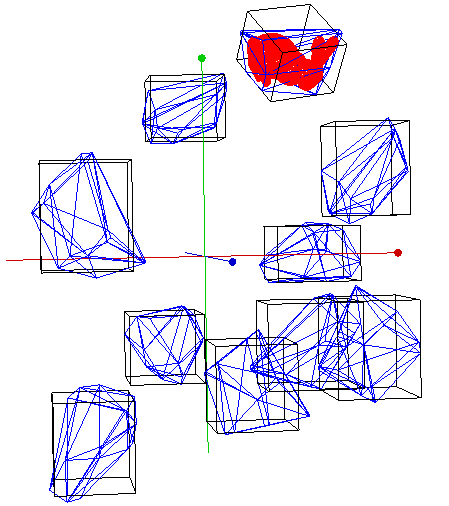
\includegraphics[width=.22\textwidth]{dynamic-bunny-m10-s2.png}
}
\subcaptionbox{$move=3$}{
  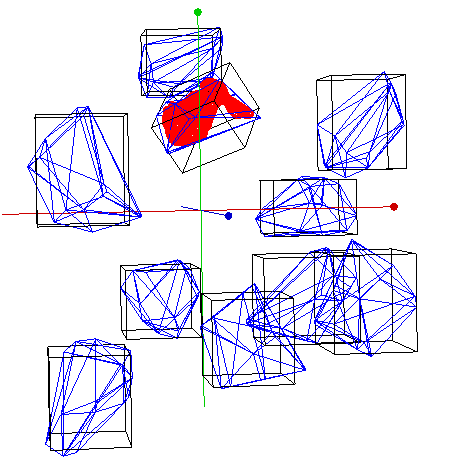
\includegraphics[width=.22\textwidth]{dynamic-bunny-m10-s3.png}
}\\ 
\subcaptionbox{$move=4$}{
  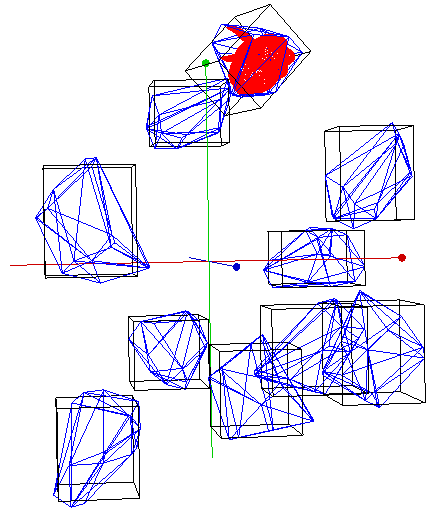
\includegraphics[width=.22\textwidth]{dynamic-bunny-m10-s4.png}
}
\subcaptionbox{$move=5$}{
  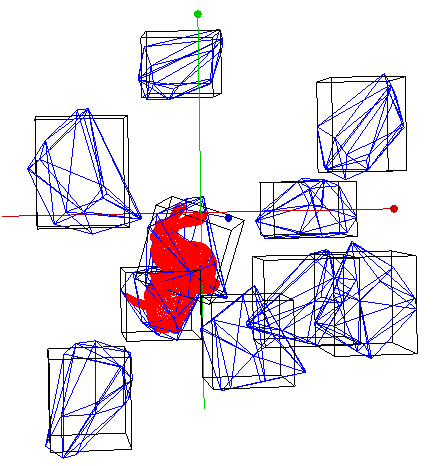
\includegraphics[width=.22\textwidth]{dynamic-bunny-m10-s5.png}
}
\subcaptionbox{$move=6$}{
  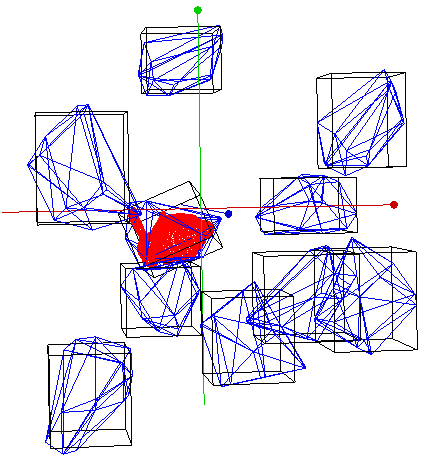
\includegraphics[width=.22\textwidth]{dynamic-bunny-m10-s6.png}
}
\subcaptionbox{$move=7$}{
  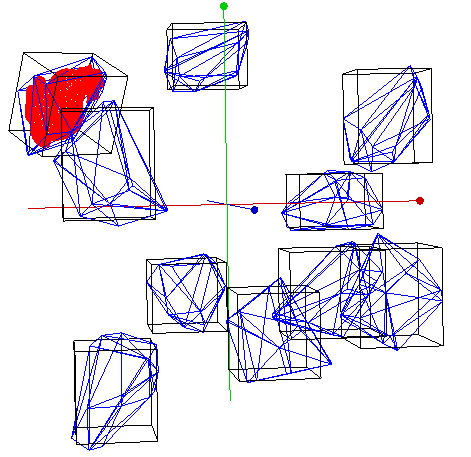
\includegraphics[width=.22\textwidth]{dynamic-bunny-m10-s7.png}
}\\
\caption{运动场景下~Bunny~模型碰撞检测示例}
\label{fig:dynamic:cd:bunny}
\end{figure}

表~\ref{tab:exper:kcbp:kdop:init:k24}~为本文算法和~$k$-DOP~算法均采用~$k$-DOP~实现中~$k=24$~默认值的初始化时间对比,init($k$-CBP)~所代表的时间表示构造~$k$-CBP~及模型
的~AABB~树所耗费的时间,init($k$-DOP)~为构造~$k$-DOP~所耗费的时间,$n$~的数量为动态碰撞检测场景中模型的总数量,从中可知本文在初始化时间上至少快~8~倍以上,同是对~10~个~Hand~模型进行初始化,
$k$-DOP~算法需要近~40~秒的时间,而本文算法仅需~4.5~秒。

\begin{table}[htbp]
\centering
\caption{本文算法与~$k$-DOP~初始化时间对比($k=24$)}
\label{tab:exper:kcbp:kdop:init:k24}
\begin{tabular}{ccccc}
\toprule[1.5pt]
\multirow{2}{*}{Model} & \multicolumn{2}{c}{$n=2$} &
\multicolumn{2}{c}{$n=10$}\\
\cmidrule(lr){2-3}\cmidrule(lr){4-5}
%~&init($k$-CBP)(ms)&init($k$-DOP)& init($k$-CBP)&init($k$-DOP) \\
~&init($k$-CBP)(ms)&init($k$-DOP)(ms)& init($k$-CBP)(ms)&init($k$-DOP)(ms) \\
\midrule[1pt]
Bunny    &17.63  &189.78   &116.59 	  &926.10   	 \\
Apple    &30.87  &749.48   &226.20 	  &3732.43  	 \\
HappyBuddha	&160.58 	&2557.27 	&1361.57 	&12663.13  \\
Dinosaur &250.55 &4281.15  &2230.88	  &21493.08 	 \\
Hand	&506.98 &	7926.88 &	4478.18 &	39538.70 \\ 
\bottomrule[1.5pt]
\end{tabular}
\end{table}

在运动环境中,本文算法与$k$-DOP~算法初始化过程与在静态环境中一样,$k$-DOP~需要构造~$k$-DOP~树也因此耗费很多时间,本文需要构造~AABB~树,也是初始化过程中占用时间较多的步骤。图~\ref{fig:chart:exps:kdop:kcbp:k24:dynamic}~为运动场景下本文算法与~$k$-DOP~实验结果对比,其中凸包围多面体面数~$k=24$。
横坐标表示其中一个模型运动的步数~$moves$,纵坐标表示随机运动~$moves$~步碰撞检测所耗费的时间,实心圆所代表曲线为前文提出的基于~GJK~算法实现,空心圆为基于~$k$-DOP~实现,另外的为前文提出的基于~AABB~树实现。

\begin{figure}[htbp] 
\centering
\subcaptionbox{Bunny(4968个三角网格)\label{fig:exp:dynamic:bunny}}
{  
   \includegraphics[width=\fourgraphicswidth\textwidth,page=2]{dynamiccd.pdf}
}
\subcaptionbox{Apple(8040个三角网格)\label{fig:exp:dynamic:apple}}
{  
    \includegraphics[width=\fourgraphicswidth\textwidth, page=4]{dynamiccd.pdf}
}\linebreak %强制换行
\subcaptionbox{HappyBuddha(50000个三角网格)\label{fig:exp:dynamic:happyBuddha}}
{  
   \includegraphics[width=\fourgraphicswidth\textwidth, page=13]{dynamiccd.pdf}
}
%\subcaptionbox{Dinosaur(64546个三角网格)\label{fig:exp:dynamic:dinosaur}}
%{  
%   \includegraphics[width=\fourgraphicswidth\textwidth, page=6]{dynamiccd.pdf}
%}
\subcaptionbox{Hand(128314个三角网格)\label{fig:exp:dynamic:hand}}
{  
   \includegraphics[width=\fourgraphicswidth\textwidth, page=15]{dynamiccd.pdf}
}

\caption{运动场景下本文算法与~$k$-DOP~实验结果对比($k=24,n=2$)}
\label{fig:chart:exps:kdop:kcbp:k24:dynamic}
\end{figure}

在~Bunny~模型中,本文基于~GJK~算法耗时最少,基于~$k$-DOP~算法耗时最久,本文基于~AABB~算法居中,总体趋势为~$moves$~越大,耗时也越久,表~\ref{tab:exp:bunny:k24:kdop:kcbp:detail:dynamic}~
为~2~个~Bunny~模型在随机运动~$moves$~步和~$k$-DOP~算法的比较结果,当真实模型相交数量较多时,三种算法所耗费的时间也更多,总体来看本文算法是基于~$k$-DOP~耗时的~0.8--3.75~倍。

\begin{table}[htbp]  
\centering
\caption{运动场景下本文算法与~$k$-DOP~实验结果(Bunny)}
\label{tab:exp:bunny:k24:kdop:kcbp:detail:dynamic}
\begin{tabular}{cccccc}
\toprule[1.5pt]
$moves$ & DT($k$-CBP)(AABB) &DT($k$-DOP) & DT($k$-CBP)(GJK) & DP($k$-CBP) & DP(Model) \\
\midrule[1.0pt]
10  &   0.00  &	  0.40 & 	0.01&  0	& 0 \\
50  &   0.80  &	  0.20 & 	0.01&  0	& 0 \\
100 &   3.40  &	  1.60 & 	2.00&  4	& 4 \\
200 &   2.60  &	  2.20 & 	1.00&  1	& 1 \\
300 &   3.60  &	  3.00 & 	0.80&  2	& 2 \\
400 &   6.40  &	  4.20 & 	1.80&  8	& 6 \\
500 &   6.80  &	  5.40 & 	3.00&  11	& 8 \\
600 &   13.60 &   6.20 & 	6.40&  10	& 8 \\
700 &   10.80 &   8.40 & 	5.00&  14	& 8 \\
800 &   12.60 &   8.20 & 	3.40&  10	& 8 \\
900 &   10.00 &   9.20 & 	3.20&  9	& 7 \\
1000&   16.00 &   11.40&	6.40&  22	& 17 \\
\bottomrule[1.5pt]
\end{tabular}
\end{table}

随着三角网格增多,三种算法所耗费时间均有所增加,总体而言,基于~$k$-DOP~的算法比较稳定,而本文算法随着模型不同波动较大。

%如图~\ref{fig:exp:dynamic:budda}~所示的~Budda~模型,本文的两种算法耗时较一致,因为两种算法在~$k$-CBP~相交后均依赖于模型基于~AABB~树的碰撞检测算法。实际上,最终碰撞检测耗时与在运动过程中相交的次数有关,且同时也与相交位置有关。
%图~\ref{fig:exp:dynamic:budda}~所示的~Budda~模型在~$moves=700$~时,均耗时200多毫秒,因为此时$k$-CBP~相交对数为~DP($k$-CBP)$=10$,且实际模型相交对数为5,且在这5次模型真实相交过程中,调用单独包围盒和旋转包围盒碰撞检测算法最大达46044次,且三角网格相交测试数量也达到8040次,因此总体耗时很久,深究原因发现~Budda~模型的底部包含有很多极小的共面三角形,导致很多这些极小的共面三角形与其他三角形发生多次碰撞检测,这表明本文算法存在一定鲁棒性问题。
%原因是共面的三角形很多,budda-long-time-ui2.png 三角形包围盒都相交但三角形不相交。

\begin{figure}[htbp] 
\centering
\subcaptionbox{Bunny(4968个三角网格)\label{fig:exp:dynamic:m10:bunny}}
{  
   \includegraphics[width=\fourgraphicswidth\textwidth,page=7]{dynamiccd.pdf}
}
\subcaptionbox{Apple(8040个三角网格)\label{fig:exp:dynamic:m10:apple}}
{  
    \includegraphics[width=\fourgraphicswidth\textwidth, page=8]{dynamiccd.pdf}
}\linebreak %强制换行
\subcaptionbox{HappyBuddha(50000个三角网格)\label{fig:exp:dynamic:m10:happyBuddha}}
{  
   \includegraphics[width=\fourgraphicswidth\textwidth, page=14]{dynamiccd.pdf}
}
%\subcaptionbox{Dinosaur(64546个三角网格)\label{fig:exp:dynamic:m10:dinosaur}}
%{  
%   \includegraphics[width=\fourgraphicswidth\textwidth, page=10]{dynamiccd.pdf}
%}
\subcaptionbox{Hand(128314个三角网格)\label{fig:exp:dynamic:m10:hand}}
{  
   \includegraphics[width=\fourgraphicswidth\textwidth, page=16]{dynamiccd.pdf}
}
\caption{运动场景下本文算法与~$k$-DOP~实验结果对比($k=24,n=10$)}
\label{fig:chart:exps:kdop:kcbp:k24:m10:dynamic}
\end{figure}

当模型数量~$n$~的值增大时,三种算法整体趋势仍能保持一致,如图~\ref{fig:chart:exps:kdop:kcbp:k24:m10:dynamic}~所示为相同~$k$~值,相同运动路径(包括平移距离旋转角度以及运动步数)下~10~个模型下的碰撞检测结果。
%对于~Budda~模型,本文算法仍耗时较久,原因与~$n=2$~时一致,即~$k$-CBP~相交,用~AABB~树进行模型的碰撞检测时,树形结构遍历较多且到叶子节点三角网格测试的次数也较多。
本文基于~$k$-CBP~的两种碰撞检测算法步调一致,如~Hand~模型在~$moves=700$~时都耗时较久,因为两种算法在~$k$-CBP~相交后,都是利用~AABB~树进行对真实模型的碰撞检测,且此时~AABB~包围盒节点相交检测较多,达到~5~万多次,因此耗时较久。
整体来看,在运动场景的碰撞检测环境中,本文基于$k$-CBP~结合~GJK~的算法在一定程度上有一定优势,而基于$k$-DOP~算法相对较稳定,但其初始化时间很长。

\begin{figure}[htbp] 
\centering
\subcaptionbox{Bunny(4968个三角网格)\label{fig:exp:static:k24:k46:bunny:dynamic}}
{  
   \includegraphics[width=\fourgraphicswidth\textwidth,page=11]{dynamiccd.pdf}
}
\subcaptionbox{Apple(8040个三角网格)\label{fig:exp:static:k24:k46:apple:dynamic}}
{  
    \includegraphics[width=\fourgraphicswidth\textwidth, page=12]{dynamiccd.pdf}
}
\caption{运动场景下不同~$k$~值实验结果对比}
\label{fig:chart:exp:kdop:kcbp:k24:k46:dynamic}
\end{figure}

与在静止场景的碰撞检测环境一样,在运动场景的碰撞检测环境中,更大的~$k$~值也不一定能够使碰撞检测的效率提高,仍以~Bunny~模型和~Apple~模型为例(模型数量~$n=10$),
如图~\ref{fig:chart:exp:kdop:kcbp:k24:k46:dynamic}~为~$k=24$~和~$k=46$~的结果对比,其中,虚线的结果为~$k=46$~的结果,实线为~$k=24$~的结果,看出三种算法在~$k=24$~时碰撞检测所耗费的时间更少。因此在实际应用环境中应该根据具体的碰撞检测环境
选择不同的~$k$~值。

\section{本章小结}
\label{sec:chap03:summary}

本章主要介绍了基于~$k$-CBP~的碰撞检测算法,该算法主要利用包围盒和~$k$-CBP~对模型进行过滤,尽早排除不可能相交的模型。
本文利用基于~AABB~树的方法和~GJK~的算法进行~$k$-CBP~之间的相交检测,在模型的~$k$-CBP~相交后,继续利用模型的~AABB~树对原始模型进行碰撞检测。
本章基于~$k$-CBP~的碰撞检测实验从三个角度进行,一方面与仅用包围盒过滤算法进行对比,另外分别从静止和运动场景中与基于~$k$-DOP~的算法进行对比,
实验结果表明本文算法能够有效加速碰撞检测过程。

